\documentclass[12pt]{article}

\usepackage[]{graphicx}
\usepackage[]{color}
\usepackage{alltt}

\newcommand{\mytitle}{fANOVA for Interpretable Machine Learning}
\newcommand{\myname}{Juliet Fleischer}
\newcommand{\mysupervisor}{Prof. Dr. Thomas Nagler}

\usepackage[a4paper, width = 160mm, top = 35mm, bottom = 30mm, 
bindingoffset = 0mm]{geometry}
\usepackage{setspace}
\onehalfspacing
\usepackage[utf8]{inputenc}
\usepackage{amssymb}
\usepackage{amsmath}
\usepackage{adjustbox}
\usepackage{ragged2e}
\usepackage{xcolor}
\usepackage[round, comma]{natbib}
\usepackage{fancyhdr}
\usepackage{textcmds}
\newcommand{\changefont}{%
    \fontsize{8}{11}\selectfont
}
\usepackage{amsthm}
\newtheorem{proposition}{Proposition}[section]
\newtheorem{definition}{Definition}[section]
\newtheorem{lemma}{Lemma}[section]
\newtheorem{theorem}{Theorem}[section]
\usepackage{hyperref}
\hypersetup{
  colorlinks = true,
  linkcolor = black,
  urlcolor = black,
  citecolor = black}
\pagestyle{fancy}
\fancyhead{}
\fancyhead[R]{\changefont{\mytitle}}
\fancyfoot{}
\fancyfoot[R]{\thepage}
\setlength{\headheight}{14.5pt}
\setlength{\parindent}{0pt}
\interfootnotelinepenalty = 10000

% ------------------------------------------------------------------------------
% MAIN -------------------------------------------------------------------------
% ------------------------------------------------------------------------------
\IfFileExists{upquote.sty}{\usepackage{upquote}}{}
\begin{document}

% FRONT PAGE -------------------------------------------------------------------
 
\begin{titlepage}
\begin{center}
    
\LARGE
Bachelor's Thesis
    
\vspace{0.5cm}
      
\rule{\textwidth}{1.5pt}
\LARGE
\textbf{\mytitle}
\rule{\textwidth}{1.5pt}
   
\vspace{0.5cm}
      
\large
Department of Statistics \\
Ludwig-Maximilians-Universität München 

\vfill

\Large
\textbf{\myname}

\vfill

\large
Munich, Month Day\textsuperscript{th}, Year
      
\vfill


\includegraphics[width = 0.4\textwidth]{sigillum.png}

\vfill

\normalsize
Submitted in partial fulfillment of the requirements for the degree of B. Sc.
\\

Supervised by \mysupervisor

\end{center}
\end{titlepage}

% CONTENTS ---------------------------------------------------------------------

\pagenumbering{Roman}
\newpage

\begin{abstract}

Lorem ipsum dolor sit amet, consectetur adipiscing elit, sed do eiusmod tempor 
incididunt ut labore et dolore magna aliqua. Ut enim ad minim veniam, quis 
nostrud exercitation ullamco laboris nisi ut aliquip ex ea commodo consequat. 
Duis aute irure dolor in reprehenderit in voluptate velit esse cillum dolore eu 
fugiat nulla pariatur. Excepteur sint occaecat cupidatat non proident, sunt in 
culpa qui officia deserunt mollit anim id est laborum.

\end{abstract}

\newpage
\tableofcontents

%%%% if you would want to include material overview
%%%% use one of the following in addition
% \newpage
% \listoffigures
% \newpage
% \listoftables
\newpage

% CHAPTERS ---------------------------------------------------------------------

\pagenumbering{arabic}
    
\section{Introduction}
\label{intro}
% The mathematics of cooperation and attribution.

\subsection*{Questions}
\subsubsection*{Clarifying the connection between fANOVA, expected value, and projection \& bringing together different definitions}
When I start from \cite{muehlenstaedt2012} and basically go the way: \textit{fANOVA term $\rightarrow$ expected value $\rightarrow$ projection}, I arrive at the formulation where we first compute the projection and afterwards subtract lower order terms. For example following the definition by \cite{muehlenstaedt2012} and using the parallel between (conditional) expected value and the projection \citep{vanravenzwaaij2018} we can write for example for $u = \{1,2\}$:
\begin{align*}
    y_{12}(.;.) &:= \mathbb{E}[y(\boldsymbol{X}) \mid X_1, X_2] - y_\emptyset - y_{\{1\}}(\cdot) - y_{\{2\}}(\cdot) \\
    &= \arg\min_{g_{\{1,2\}} \in \mathcal{G}_{\{1,2\}}} \mathbb{E}\left[(y(\boldsymbol{X}) - g_{\{1,2\}}(X_1, X_2))^2\right] - y_\emptyset - y_{\{1\}}(\cdot) - y_{\{2\}}(\cdot) \\
    &= (\Pi_{\mathcal{G}_{\{1,2\}}}y)(.;.) - y_\emptyset - y_{\{1\}}(\cdot) - y_{\{2\}}(\cdot)
\end{align*}

But when I get it correctly \cite{hooker2007} writes his generalized fANOVA components as the projection of the differences. Also, he goes the other way around, starting from the projections (and we could restate this as the conditional expected value).

Because Hooker defines the fANOVA terms as:
\begin{equation}
\left\{ f_u(x_u) \,\middle|\, u \subseteq d \right\}
= \arg\min_{\{g_u \in L^2(\mathbb{R}^u)\}_{u \subseteq d}} 
\int \left( y(\boldsymbol{x}) - \sum_{u \subseteq d} g_u(x_u) \right)^2 w(\boldsymbol{x}) \, d\boldsymbol{x}
\label{eq:fanova_decomposition_generalized}
\end{equation}

And I think we can rewrite this as the conditional expected value. For example for $u = \{1,2\}$:
\begin{align*}
    y_{12}(.;.) &:= \arg \min_{g_{\{1,2\}} \in L^2(\mathbb{R}^2)} \int \left( y(\boldsymbol{x}) - \sum_{\{1,2\}} g_{\{1,2\}}(.;.) \right)^2 w(\boldsymbol{x}) \, d\boldsymbol{x} \\
    &= \arg \min_{g_{\{1,2\}} \in L^2(\mathbb{R}^2)} \int \left( y(\boldsymbol{x}) - y_\emptyset - y_{\{1\}}(\cdot) - y_{\{2\}}(\cdot) - g_{\{1,2\}}(.;.) \right)^2 w(\boldsymbol{x}) \, d\boldsymbol{x} \\
    &= \arg \min_{g_{\{1,2\}} \in L^2(\mathbb{R}^2)} \mathbb{E}[(y(\boldsymbol{X}) - y_\emptyset - y_{\{1\}}(X_1) - y_{\{2\}}(X_2) - g_{\{1,2\}}(X_1, X_2))^2] \\
    &= (\Pi_{\mathcal{G}_{\{1,2\}}}(y - y_\emptyset - y_{\{1\}}(\cdot) - y_{\{2\}}(\cdot)))(.;.) \\
    &= \mathbb{E}[y(\boldsymbol{X}) - y_{\emptyset} - y_{\{1\}}(X_1) - y_{\{2\}}(X_2) | X_1 = x_1, X_2 = x_2]
\end{align*}

So \cite{hooker2007} defines the fANOVA terms via the projection \textit{fANOVA term $\rightarrow$ projection $\rightarrow$ expected value (not in Hooker)}. But he takes the projection of the differences. 

\begin{itemize}
    \item Could it happen that based on fANOVA decomposition we build a model which uses the interaction effect of $i,j$ but not the main effects $i$ and/or $j$? 
    \item Can I really compute the generalized fANOVA terms a proposed by \cite{hooker2007} by hand? \href{https://christophm.github.io/interpretable-ml-book/decomposition.html}{Molnar} writes: ``The estimation is done on a grid of points in the feature space and is stated as a minimization problem that can be solved using regression techniques. However, the components cannot be computed independently of each other, nor hierarchically, but a complex system of equations involving other components has to be solved. The computation is therefore quite complex and computationally intensive.'' \textit{If he would write he generalized fANOVA as conditional expected values it is actually not that complicated and we simply would need to solve regression problems hierarchically.}
    \item I am still confused if setting the zero-mean constraint for $X_i \overset{\text{i.i.d.}}{\sim} \mathcal{U}[0, 1]$ is essentially saying that we centre the distribution and now assume $X_i \overset{\text{i.i.d.}}{\sim} \mathcal{U}[-1, 1]$. So can we, instead of explicitly stating the zero-mean constraint just assume $X_i \overset{\text{i.i.d.}}{\sim} \mathcal{U}[-1, 1]$? And following the same principle we would shift other distributions by altering their parameters, not by explicitly stating the zero-mean constraint? Then for the standard normal distribution we wouldn't need to do anything, it is already centred around 0. For other distributions we would need to change, and for some it doesn't make inhaltlichen Sinn e.g. Poisson distribution? \textit{No generally zero-mean constraint and distribution assumption of the variables has no connection. The zero-mean constraint is sth. we set for the fANOVA terms $y_u$ while distribution assumption is about the input variables $X_i$. We don't set the zero-mean constraint for the variables"}
    \item 
    \item fANOVA decomposition via the integral, how would the zero mean constraint look here? (see ``General\_fANOVA\_handnotes'')
    \item Can you reconstruct the function from only the fANOVA terms? I think it can be reconstructed only if variables are independent, have zero-mean, are orthogonal?
    \item Is it possible to perform fANOVA for non-square-integrable functions? \textit{in general yes but the variance decomposition doesn't work then or might have problems.}
    \item fANOVA decomposition for discrete variables possible? Does it make sense even?
    % \item Denote original model with $y$ or $f$?
    \item Connection between the (conditional) expected value, (partial) integral, projections (section~\ref{general_definitions})?
    \item In the hierarchical orthogonality condition (4.2) formulated in \cite{hooker2007} for the gerneralized fAVNOA framework, shouldn't we explicitly exclude the case that $v = u$, because then, we would require that the inner product of the fANOVA component is zero wouldn't we (section~\ref{generalization})?
    % \item If the general fANOVA formulation is a true generalization then I should be able to take the general form and construct from it the simple form when I use certain constrains (such as independence, uniform distribution, etc.) right?
    \item Why is it a problem, when explainability methods also place large emphasis on regions of low probability mass when dependencies between variables exist - because in the end explainability is about explaining the model, not the data generating process; and after all it is how the model works in these regions. [But as the Hooker example illustrates, how the model works and what it estimates in these regions is wrong and then it's better to not report any model behaviour or come closer to the DGP than to give wrong estimations?]
    \item 
    \item Use of AI tools?
    \item Do we need to restrict ourselves to the unit hypercube? Or does fANOVA decomposition work in general, but maybe with some constraints? Originally it was constructed for models on the unit hypercube $[0,1]$, but other papers also use models from $R^d$ \textit{Generally no restriction, so next step could be to generalize, to $\mathbb{R}^n$, other measures, dependent variables}
    \item Still unclear: Are the terms fully orthogonal or hierarchically? See subsection on Orthogonality of the fANOVA terms (especially the example) I think in the original fANOVA decomposition the terms are orthogonal but in the generalized fANOVA \citep{hooker2007} they are hierarchically orthogonal. \textit{fully orthogonal when independence assumption, probably partially when no independence}
    \item $x_1, \dots, x_k$ are simply the standardized features, right? \textit{Yes}
    \item {\color{orange}My current understanding: we need independence of $x_1, \dots x_k$ so that fANOVA decomposition is unique (and orthogonality holds). We need zero-mean constraint for the orthogonality of the components. We need orthogonality for the variance decomposition.}\textit{zero-mean $\rightarrow$ orthogonality $\rightarrow$ uniqueness; Lemma 1 im Hooker 2007 ist verallgemeinerg ds zero-mean constraint}
    \item Next step might be to investigate the (mathematical) parallels of fANOVA decomposition and other IML methods (PDP, ALE, SHAP), e.g. there is definitely a strong relationship between Partial dependence (PD) and fANOVA terms, and PD is itself again related to other IML methods; Also look how are other IML models studied and study fANOVA in a similar way (e.g. other IML methods are defined, checked for certain properties, examined under different conditions (dependent features, independent features) etc.) (see dissertation by Christoph Molnar for this); Also I would be very interested in investigating the game theory paper further \citep{fumagalli2025} but still a bit unsure if it is too complex.
    \item Why does a fANOVA decomposition of a simple GAM not lead to the ``true'' coefficients? \href{https://christophm.github.io/interpretable-ml-book/decomposition.html}{https://christophm.github.io/interpretable-ml-book/decomposition.html} talks about this a bit in the subchapter ``Statistical regression models'' \textit{It should actually lead to the GAM; at least under all the constraint like zero-mean constraint and orthogonality}
    \item 
    \item In \cite{hooker2004} they work with $F(x)$ and $f(x)$, but in \cite{sobol2001} they only work with $f(x)$. I think this is only notation? \textit{Only notation.}
    \item Does orthogonality in fANOVA context mean that all terms are orthogonal to each other? Or that a term is orthogonal to all lower-order terms (\ldq Hierarchical orthogonality \rdq)? \textit{The terms are hierarchically orthogonal, so each term is orthogonal to all lower-order terms, but not to the same-order terms! So $f_1$ is not necessarily orthogonal to $f_2$ but it is orthogonal to $f_{12}$, $f_{0}$.} 
    \item Do the projections here serve as approximations? (linalg skript 2024 5.7.4 Projektionen als beste Annäherung) \textit{Yes, they can be interpreted as sort of approximation.}
    \item Which sub-space are we exactly projecting onto? Are the projections orthogonal by construction (orthogonal projections) or only when the zero-mean constraint is set? \textit{The subspace we project onto depends on the component. For $f_0$ we project onto the subspace of constant functions, for $f_1$ we project onto the subspace of all functions that involve $x_1$ and have an expected value of 0 (zero-mean constraint to ensure orthogonality). It depends on the formulation of the fANOVA decomposition if you need to explicitly set the zero-mean constraint for orthogonality or if it is met by construction.}
    \item How \ldq far\rdq should I go back, formally introduce $L^2$ space, etc. or assume that the reader is familiar with it? \textit{Yes, space, the inner product on this space should be formally introduced.}
    % \item zero mean condition vs. zero-sum condition: according to GPT zero mean condition is related to orthogonality and zero-sum to the additivity
\end{itemize}

% \section*{fANOVA Brainstorming Questions}

% \subsection*{What happens if...?}
% \begin{itemize}
%     \item What happens if the function \( f \) is linear in all its variables? What do the fANOVA terms look like in that case?
%     \item What happens if some variables are independent? Do any Sobol’ terms vanish automatically?
%     \item What happens if you permute the inputs? Do the Sobol’ indices change?
%     \item What happens if two variables are strongly collinear? How does that affect the interpretability of fANOVA?
% \end{itemize}

% \subsection*{Why is...?}
% \begin{itemize}
%     \item Why is orthogonality (zero mean and mutual independence of components) important in fANOVA?
%     \item Why is the constant term \( f_0 \) equal to the expected value of \( f \)?
%     \item Why is fANOVA usually associated with variance-based methods like Sobol indices?
%     \item Why is it necessary to subtract lower-order terms when computing higher-order ones?
%     \item Why is the decomposition hierarchical?
% \end{itemize}

% \subsection*{Is it possible to...?}
% \begin{itemize}
%     \item Is it possible to compute fANOVA in closed form for certain functions (e.g., polynomials)?
%     \item Is it possible to use fANOVA in models where inputs are dependent?
%     \item Is it possible to extend fANOVA to time-series models or dynamic systems?
%     \item Is it possible to use fANOVA ideas in neural networks? How would you interpret interactions then?
% \end{itemize}

% \subsection*{What does this remind you of? (Analogies and Parallels)}
% \begin{itemize}
%     \item fANOVA reminds me of \emph{Fourier decomposition}: projecting a function onto orthogonal basis functions.
%     \item It feels similar to \emph{PCA}, but in the input space instead of the output space.
%     \item fANOVA terms are like \emph{partial derivatives} in symbolic differentiation — quantifying localized influence.
%     \item It’s analogous to \emph{ANOVA in statistics}, but instead of experimental groups, you decompose function behavior.
%     \item In machine learning, it reminds me of \emph{feature importance} in random forests or \emph{Shapley values}.
%     \item fANOVA’s additive structure is similar to \emph{GAMs (Generalized Additive Models)}.
% \end{itemize}

% \subsection*{How does fANOVA compare to...?}
% \begin{itemize}
%     \item How does fANOVA compare to Shapley values? (Shapley is axiomatic, fANOVA is Hilbert space projection-based.)
%     \item How does fANOVA compare to LIME/SHAP in interpretability?
%     \item How does fANOVA compare to gradient-based sensitivity methods?
%     \item How does fANOVA compare to partial dependence plots?
%     \item How does fANOVA compare to mutual information as a dependence measure?
% \end{itemize}

\newpage

\section{Background Knowledge}
\label{background}
% Prerequesites:
% L2 space, Hilbert space
% inner product, norm
% orthogonal projections
% expected value, conditional expected value
\subsection*{Basic Setup}
Let $(\Omega, \mathcal{F}, \nu)$ be a measure space, where $\Omega$ is a sample space, $\mathcal{F}$ is a $\sigma-$algebra on $\Omega$ and $\nu: \mathcal{F} \rightarrow [0, 1]$ is a probability measure. $\mathcal{B}^N$ is the Borel $\sigma$-algebra on $\mathbb{R}^N, N \in \mathbb{N}$.
$\boldsymbol{X} = (X_1, \dots, X_N): (\Omega, \mathcal{F}) \rightarrow (\mathbb{R}^N, \mathcal{B}^N)$ denotes a $\mathbb{R}^N$-valued random vector.\par
We assume that the probability distribution of $\boldsymbol{X}$ is continuous and completely defined by the joint probability density function (pdf) $f_{\boldsymbol{X}}: \mathbb{R}^N \rightarrow \mathbb{R}_{0}^+$. $f_{\boldsymbol{X}}$ is the pdf w.r.t. measure $\nu$. \par

Let $u$ denote a subset of indices $\{1, \dots, N\}$, and $-u := \{1, \dots, N\} \backslash{} u$ its compliment.
$\boldsymbol{X_u} = (X_1, \dots, X_{|u|}), u \neq \emptyset, 1 \leq i_1 < \dots < i_{|u|} \leq N$ is a sub-vector of $\boldsymbol{X}$ and $\boldsymbol{X}_{-u} = \boldsymbol{X}_{\{1, \dots, N\} \backslash{} u}$ is the complement of $\boldsymbol{X}_u$.\par

The marginal density function is $f_u(\boldsymbol{x_u}) := \int f_{\boldsymbol{X}}(\boldsymbol{x})d\boldsymbol{x_{-u}}$ for a given set $\emptyset \neq u \subseteq \{1, \dots N\}$.
$f(\boldsymbol{X}) := f(X_1, \dots, X_N)$ is a mathematical model with random variables as inputs.
We write a vector space of square-integrable functions as
\[\mathcal{L}^2(\Omega, \mathcal{F}, \nu) = \left\{ f: \Omega \rightarrow \mathbb{R} \; \textit{s.t.} \; \mathbb{E}[f^2(\boldsymbol{X})] < \infty \right\}\].
% = \left\{ f(x) : \mathbb{R}^{n} \to \mathbb{R}, \; \textit{s.t.} \; \int f^2(x)\, d\nu(x) < \infty \right\}

$\mathcal{L}^2(\Omega, \mathcal{F}, \nu)$ is a Hilbert space with the inner product defined as:
\[
\langle f, g \rangle = \int f(\boldsymbol{x}) g(\boldsymbol{x}) \, f_{\boldsymbol{X}}d\nu(\boldsymbol{x}) = \mathbb{E}[f(\boldsymbol{X})g(\boldsymbol{X})].
\]
The norm is denoted as $\|.\| $ and defined by:
\[
\|f\| = \sqrt{\langle f, f \rangle} = \sqrt{\int f^2(x) \, d\nu(x)} = \mathbb{E}[f^2], \quad \forall f \in \mathcal{L}^2.
\]

We denote strict inclusion by $\subsetneq$ and $\subset$ allows for equality.
% We write captial letters for random variables, lower case letters for realizations of random variables, bold for multidimensional random variables, and noraml for sclar values. 
Formal setup now based on \cite{chastaing2012,rahman2014}.
{\color{blue} Maybe also cite: \href{https://apachepersonal.miun.se/~andrli/Bok.pdf}{https://apachepersonal.miun.se/~andrli/Bok.pdf}; also look again at pdf and measure setup.}

\subsection*{Orthogonal projection}
Let $\mathcal{G} \subset \mathcal{L}^2$ denote a linear subspace. The projection of $f$ onto $\mathcal{G}$ is defined by the function $\Pi_{\mathcal{G}}f$ which minimizes the distance to $f$ in $\mathcal{L}^2$:
\[
\Pi_{\mathcal{G}}f = \arg\min_{g \in \mathcal{G}} \|f - g\|^2
= \arg\min_{g \in \mathcal{G}} \mathbb{E}[(f - g)^2].
\]

Definition of $\mathcal{L}^2$ space and projection modified from \href{https://tnagler.github.io/mathstat-lmu-2024.pdf}{https://tnagler.github.io/mathstat-lmu-2024.pdf}.

% conditional expectation defined via integral conditioned on certain value/ partial integral


\subsection*{Unconditional and Conditional expectation}
$\mathbb{E}[.]$ denotes the expectation operator, $Var[.] := \mathbb{E}[(. - \mathbb{E}[.])^2]$ denotes the variance and $Cov[.,*] := \mathbb{E}[(. - \mathbb{E}[.]) (* - \mathbb{E}[*])]$ denotes the covariance operator.\par
In general, we define the conditional expectation of a vector of random variables $\boldsymbol{X} = (X_1, X_2)$ as follows:
\[
\mathbb{E}[g(X_1, X_2) \mid X_1 = x_1] = \int g(x_1, s_2) \, p_{X_2 \mid X_1}(s_2 \mid x_1) \, ds_2.
\]
Only when $X_1$ and $X_2$ are independent can we write
\begin{align*}
    \mathbb{E}[g(X_1, X_2) \mid X_1 = x_1] = \int g(x_1, s_2) \, p_{X_2 \mid X_1}(s_2 \mid x_1) \, ds_2 = \int g(x_1, s_2) \, p_{X_2}(s_2) \, ds_2 = \mathbb{E}_{X_2}[g(x_1, X_2)].
\end{align*}

Extended to $n$ random variables it looks as follows. Without loss of generality, we condition on $X_1 = x_1$:
\begin{align*}
    \mathbb{E}[g(X_1, \dots, X_n) \mid X_1 = x_1] &= \int g(x_1, s_2, \dots, s_n) \, p_{X_2, \dots, X_n \mid X_1}(s_2, \dots, s_n \mid x_1) \, ds_2 \dots ds_n \\
    &= \int g(x_1, s_2, \dots, s_n) \, p_{X_2}(s_2, \dots, s_n) \, ds_2 \dots, ds_n \\
    &= \mathbb{E}_{X_2, \dots, X_n}[g(x_1, X_2, \dots, X_n)]
\end{align*}



\subsection*{Properties of the Multivariate Normal Distribution}

Let $\boldsymbol{X} = (X_1, \dots, X_d)^\top \sim \mathcal{N}(\boldsymbol{\mu}, \boldsymbol{\Sigma})$ be a $d$-dimensional multivariate normal (MVN) random vector, where $\boldsymbol{\mu} \in \mathbb{R}^d$ is the mean vector and $\boldsymbol{\Sigma} \in \mathbb{R}^{d \times d}$ is the symmetric positive semi-definite covariance matrix.\par

The marginal distribution of $X_i$ is generally given by an univariate normal distribution:
\[
 X_i \sim \mathcal{N}(\mu_i, \Sigma_{ii}) \quad \text{for all } i = 1, \dots, d.
\]
If we condition on a subset of the variables, we can also make statements about the conditional distribution. For this we partition the random vector $\boldsymbol{X}$ into two parts, $\boldsymbol{X}_A$ and $\boldsymbol{X}_B$, where $\boldsymbol{X}_A$ contains the variables we condition on and $\boldsymbol{X}_B$ contains the remaining variables. The joint distribution of $\boldsymbol{X}$ can be expressed as:
    \[
    \boldsymbol{X} = 
    \begin{pmatrix}
    \boldsymbol{X}_A \\
    \boldsymbol{X}_B
    \end{pmatrix}
    \sim \mathcal{N}\left(
    \begin{pmatrix}
    \boldsymbol{\mu}_A \\
    \boldsymbol{\mu}_B
    \end{pmatrix},
    \begin{pmatrix}
    \boldsymbol{\Sigma}_{AA} & \boldsymbol{\Sigma}_{AB} \\
    \boldsymbol{\Sigma}_{BA} & \boldsymbol{\Sigma}_{BB}
    \end{pmatrix}
    \right).
    \]
The conditional distribution of $\boldsymbol{X}_B$ given $\boldsymbol{X}_A = \boldsymbol{x}_A$ is
    \[
    \boldsymbol{X}_B \mid \boldsymbol{X}_A = \boldsymbol{x}_A \sim 
    \mathcal{N} \left(
    \boldsymbol{\mu}_B + \boldsymbol{\Sigma}_{BA} \boldsymbol{\Sigma}_{AA}^{-1} (\boldsymbol{x}_A - \boldsymbol{\mu}_A),
    \boldsymbol{\Sigma}_{BB} - \boldsymbol{\Sigma}_{BA} \boldsymbol{\Sigma}_{AA}^{-1} \boldsymbol{\Sigma}_{AB}
    \right).
    \]
For normally distributed random variables, we also know that \(\text{Cov}(X_i, X_j) = 0 \text{, implies } X_i \perp X_j\).
% Lastly, for any real vector $\boldsymbol{a} \in \mathbb{R}^d$, the linear combination $\boldsymbol{a}^\top \boldsymbol{X}$ is normally distributed:
% \[
% \boldsymbol{a}^\top \boldsymbol{X} \sim \mathcal{N}(\boldsymbol{a}^\top \boldsymbol{\mu}, \boldsymbol{a}^\top \boldsymbol{\Sigma} \boldsymbol{a}).
% \]
\newpage
\section{Foundations}
\label{foundations}
% Good historical overview of fANOVA decomposition found in: Owen (2003), Takemura (1983)

\subsection{Early Work on fANOVA}
The main idea of the fANOVA decomposition is to decompose a statistical model into the sum of the main effects and interaction effects of its input variables. The underlying principle of fANOVA decomposition dates back to \cite{hoeffding1948}. In his famous paper he introduced U-statistics, along with the ``Hoeffding decomposition'', which allows to write a symmetric function of the data as a sum of orthogonal components. \cite{sobol1993sensitivity} used the same principle and applied it to deterministic mathematical models.
% Both methods involve the sum of orthogonal components and independent input variables.
He built on the originally called ``Decomposition into Summands of Different Dimension'' in \cite{sobol2001}, where he introduces Sobol indices and renames the method to the ``ANOVA-representation''. Sobol indices are now commonly used in sensitivity analysis. \cite{efron1981} use the idea of the decomposition to proof their famous lemma on jackknife variances. \cite{stone1994} mainly uses fANOVA decomposition to base smooth regression models with interactions on it and his paper is the building block for a broader body of work of fANOVA-based models {\color{blue}example citations needed}.


\subsection{Modern Work on fANOVA}
The fANOVA decomposition has a long history with roots in mathematical statistics and non-parametric estimation theory. In more recent years, the method has been rediscovered by the machine-learning community, especially in the context of interpretable machine learning (IML) and explainable AI (XAI). \cite{hooker2004} introduces the fANOVA decomposition with the goal of providing a global explanation method for black-box models. Since the assumptions of independent variables in classical fANOVA is often too restrictive in practice, \cite{hooker2007} generalizes the method to dependent variables. A recent paper by \cite{ilidrissi2025} can be seen as another approach to generalize the principle of fANOVA decomposition to dependent inputs.\par
There are specific domains of statistics, such as geostatistics, that explcitly build models on fANOVA framework (see \cite{muehlenstaedt2012} for fANOVA Kriging models). And recent work discovered interesting mathematical parallels between fANOVA and other IML methods, such as PDP \cite{friedman2001}, or Shapley values (\cite{fumagalli2025}, Herren, Owen preprint).

\cite{liu2006} use of fANOVA and sensitivity analysis for functions arising in computational finance.
\cite{owen2013} formal intro to fANOVA decomposition and generalization of Sobol indices.

\textbf{fANOVA and U-statistics, fANOVA and sensitivity analysis, fANOVA and GAMs (with interactions)}

\subsection{Formal Introduction to fANOVA}

\subsubsection*{fANOVA decomposition}
This chapter is based on the formal introductions by \cite{sobol1993sensitivity, sobol2001, hooker2004}, Owen, \cite{muehlenstaedt2012}. Where suitable we show both formulations of the fANOVA, via the integral and via the expected value.
Let $i_1, \dots , i_s$ denote a set of indices. For now, we assume that $X_i \overset{\text{i.i.d.}}{\sim} \mathcal{U}[0, 1]$ and work in the measure space $(X, \mathcal{F}, \nu) = ([0, 1]^n, \mathcal{B}([0, 1]^n), \lambda_{n})$. $\mathcal{B}([0, 1]^n)$ is the Borel $\sigma$-algebra on the n-dimensional unit interval and $\lambda_{n}$ is the n-dimensional Lebesgue measure. 
The general inner product and norm we defined earlier simplify under these assumptions.\par
The inner product under uniform distribution assumption:
\[
\langle f, g \rangle = \int f(x) g(x) \, d(x) \quad \forall f, g \in \mathcal{L}^2
\]
The norm under uniform distribution assumption:
\[
\|f\| = \sqrt{\langle f, f \rangle} = \sqrt{\int f^2(x) \, d(x)} \quad \forall f \in \mathcal{L}^2
\]

\textbf{Definition.} Let $f(x)$  be a mathematical model with input $X_i$ as described above. We can represent such a model $f$ as a sum of specific basis functions
\begin{equation}
    f(x) = f_0 + \sum_{s=1}^{n} \sum_{i_1 <...<i_s}^{n} f_{i_{1}...i_{s}} (x_{i_{1}} , ....,x_{i_{s}})
    \label{eq:fanova_decomposition}
\end{equation}

To ensure identifiability and interpretation, we set the zero-mean constraint. It requires that all effects, except for the constant terms, are centred around zero.
Mathematically this means that the effects integrate to zero w.r.t. their own variables:
\begin{equation}
    \int f_{i_{1}...i_{s}} (x_{i_{1}}, ...., x_{i_{s}}) \, d\nu (x_k) = 0 \quad \forall k = i_1, ...., i_s
    \label{eq:zero_mean_condition}
\end{equation}
% In combination with the zero-mean constraint (\autoref{eq:zero_mean_condition}),  \cite{sobol1993sensitivity} calls \autoref{eq:fanova_decomposition} initially the \ldq Expansion into Summands of Different Dimensions\rdq. In \cite{sobol2001} he renames the decomposition to the \ldq ANOVA-representation\rdq. Now, it is mostly referred to as the \ldq functional ANOVA decomposition\rdq \citep{hooker2004}.\par

% The fANOVA decomposition for a \( f(x_1, x_2, x_3, x_4) \) would look like
% \begin{align*}
%     f(x_1, x_2, x_3, x_4) &= f_0 + f_1(x_1) + f_2(x_2) + f_3(x_3) + f_4(x_4) \\
%     &+ f_{1,2}(x_1, x_2) + f_{1,3}(x_1, x_3) + f_{1,4}(x_1, x_4) + f_{2,3}(x_2, x_3) + f_{2,4}(x_2, x_4) + f_{3,4}(x_3, x_4) \\
%     &+ f_{1,2,3}(x_1, x_2, x_3) + f_{1,2,4}(x_1, x_2, x_4) + f_{1,3,4}(x_1, x_3, x_4) + f_{2,3,4}(x_2, x_3, x_4) \\
%     &+ f_{1,2,3,4}(x_1, x_2, x_3, x_4)
% \end{align*}

The individual terms that make up \autoref{eq:fanova_decomposition} are defined in the following.
To get the constant term, we take the integral of $f$ w.r.t. all variables:
\begin{equation}
    f_{0}(x) = \int f(x) d\nu(x) = \mathbb{E}[f(X)]
    \label{eq:intercapt}
\end{equation}
The constant term $f_0$ captures the overall mean of $f$ and serves as a baseline. Since the the remaining effects are centred around zero, they quantify the deviation from the overall mean.  Next, we take the integral of $y$ w.r.t. all variables except for $x_i$. This represents $f$ as the sum of the constant term and the isolated effect of one variable $x_i$ (main effect of $x_i$). This partial integral is equivalent to the expected value conditioned on the variable of interest $x_i$.
\begin{equation}
    f_0 + f_i(x_i) = \int f(x) \prod_{k \neq i} \nu (d_{x_{k}}) = \mathbb{E}[f(X) | X_i = x_i]
    \label{eq:main_effect}
\end{equation}
Following the same principle, we can take the integral of $f$ w.r.t. all variables except for $x_i$ and $x_j$. With this we capture everything up to the interaction effect of $x_i$ and $x_j$. This is equivalent to the expected value conditioned on both variables $x_i$ and $x_j$:
\begin{equation}
    f_0 + f_i(x_i) + f_j(x_j) + f_{ij}(x_i,x_j) = \int f(x) \prod_{k \neq i,j} \nu(d_{x_{k}}) = \mathbb{E}[f(X) | X_i = x_i, X_j = x_j]
    \label{eq:interaction_effects}
\end{equation}
For a successive construction of the fANOVA decomposition, we can generally write:
\begin{equation}
    \int f(x) \prod_{k \notin u} \nu(d_{x_{k}}) = \mathbb{E}[f(X) | X_u = x_u]
    \label{eq:fanova_component}
\end{equation}
With these partial integrations (or conditional expected values) we build up the fANOVA decomposition in a cumulative way. To actually see the fANOVA terms defined in isolation, it is clearer to rearrange terms. When we rearrange \autoref{eq:main_effect} we see that the main effect of $x_i$ is calculated by taking the marginal effect while explicitly accounting for what was already explained by lower-order terms, in this case the intercept:
\begin{equation}
    f_i(x_i) = \int f(x) \prod_{k \neq i} \nu(d_{x_{k}}) - f_0
    \label{eq:main_effect_rearranged}
\end{equation}
The two-way interactions can then be seen as the marginal effects of the involved variables, while accounting for all main effects and the constant term:
\begin{equation}
    f_{ij}(x_i,x_j) = \int f(x) \prod_{k \neq i,j} \nu(d_{x_{k}}) - f_0 - f_i(x_i) - f_j(x_j) 
    \label{eq:interaction_effects}
\end{equation}

Therefore, it is also common to formulate the fANOVA decomposition in the following way \citep{hooker2007,hooker2004}:
\begin{equation}
    f_u(x) = \int_{[0,1]^{d - |u|}} \left( f(x) - \sum_{v \subsetneq u} f_v(x) \right) \, d\nu(x_{-u}).
\end{equation}
This means we subtract all lower-order terms from the original function $f$ and then integrate over all the variables not in $u$ to get the effect of $x_u$. Using the linearity of the integral, we can also first take the partial integral of the original function w.r.t. all variables not in $u$ and then subtract all the lower-order terms, as we did above for the main effects and two-way interaction effects. So generally we write:
\begin{equation}
    f_u(x) = \int_{[0,1]^{d - |u|}} f(x) \, d\nu(x_{-u}) - \sum_{v \subsetneq u} f_v(x).
\end{equation}

The basis components offer a clear interpretation of the model, decomposing it into main effects, two-way interaction effects, and so on. This is why fANOVA decomposition has received increasing attention in the IML and XAI literature, holding the potential for a global explanation method of black box models.\par

\subsubsection*{Example 1}
Before moving to properties of the fANOVA decomposition, let us look at some examples.
First, we look at a simple function which takes as input the realization of two continuous independent random variables $X_1$ and $X_2$.
\[
g_{1}(x_1, x_2) = a + x_1 + 2x_2 + x_1x_2 \quad \text{for} \quad a, x_1, x_2 \in \mathbb{R}
\]
Computing the fANOVA decomposition of $g(x_1, x_2)$ by hand, we start with the constant term and make use of formulation via the expected value instead of the integral for notational simplicity:
\[
f_0 = \mathbb{E}[g_{1}(X_1, X_2)] = \mathbb{E}[a + X_1 + 2X_2 + X_1X_2] = \mathbb{E}[a] + \mathbb{E}[X_1] + 2\mathbb{E}[X_2] + \mathbb{E}[X_1X_2]
\]
Making use of the independence assumption of $x_1$ and $x_2$, the last term can be written as the product of the expected values. Additionally, given the zero-mean constraint, all terms, except for the constant, vanish and we obtain:
\[
f_0 = \mathbb{E}[a] + \mathbb{E}[X_1] + 2\mathbb{E}[X_2] + \mathbb{E}[X_1]\mathbb{E}[X_2] = a
\]
Under zero-mean constraint and independence, the main effects and the interaction effect can be computed as follows:
\begin{align*}
f_1(x_1) &= \mathbb{E}_{X_2}[g_{1}(x_1, X_2)] - f_0 \\
&= \mathbb{E}_{X_2}[a + x_1 + 2X_2 + x_1X_2] - a \\
&= x_1 + 2\mathbb{E}[X_2] + x_1\mathbb{E}[X_2] = x_1\\
f_2(x_2) &= \mathbb{E}_{X_1}[g_{1}(X_1, x_2)] - f_0 \\
&= \mathbb{E}_{X_1}[a + X_1 + 2x_2 + X_1x_2] - a \\
&= \mathbb{E}_{X_1}[X_1] + 2x_2 + x_2\mathbb{E}_{X_1}[X_1] = 2x_2\\
f_{12}(x_1, x_2) &= \mathbb{E}[g_{1}(x_1, x_2)] - f_0 - f_1(x_1) - f_2(x_2) \\
&= a + x_1 + 2x_2 + x_1x_2 - a - x_1 - 2x_2 = x_1x_2
\end{align*}

It comes as no surprise that in this simple case the fANOVA decomposition does not provide any additional insights. This is because the model consists of only linear terms, constant terms, and an interaction. We show this simple example nevertheless to illustrate at which step we use which assumption. Understanding this will be relevant for the generalization of the method to dependent inputs later on. Also, it is interesting to compare this example with only linear effects (and an interaction) to the following, which will include a non-linear effect.\par
\subsubsection*{Example 2}
We now look at the function $g_{2} = a + x_1 + x_{2}^2$ which includes a quadratic effect. We again assume $X_1 \perp X_2$. The constant fANOVA term is given by:
\begin{align*}
    &f_0 = \mathbb{E}[g_{2}(X_1, X_2)] = \mathbb{E}[a + X_1 + X_{2}^2] = a + \mathbb{E}[X_1] + \mathbb{E}[X_{2}^2] = a + \frac{1}{12} \\
    &\text{This works because we are still in the setting, in which we assume } X_i \overset{\text{i.i.d.}}{\sim} \mathcal{U}[0, 1], \\
    &\text{in combination with the zero-mean constraint this allows us to state:} \\
    &\mathbb{E}[X_2^2] = \mathbb{V}[X_2] = \frac{1}{12}(1 - 0)^2 = \frac{1}{12} \\
    &\text{Next, we write the main effects:} \\
    &f_1(x_1) = \mathbb{E}_{X_2}[g_{2}(x_1, X_2)] - f_0 = \mathbb{E}_{X_2}[a + x_1 + X_{2}^2] - f_0 \\
    &= a + x_1 + \mathbb{E}[X_{2}^2] - f_0 = a + x_1 + \frac{1}{12} - \left( a + \frac{1}{12} \right) = x_1 \\
    &f_2(x_2) = \mathbb{E}_{X_1}[g_{2}(X_1, x_2)] - f_0 = \mathbb{E}_{X_1}[a + X_1 + x_{2}^2] - f_0 \\
    &= a + \mathbb{E}[X_1] + x_{2}^2 - f_0 = a + x_{2}^2 - \left( a + \frac{1}{12} \right) = x_{2}^2 - \frac{1}{12} \\
    &\text{Finally, we compute the interaction effect:} \\
    &f_{12}(x_1, x_2) = \mathbb{E}[g_{2}(x_1, x_2)] - f_0 - f_1(x_1) - f_2(x_2) \\
    &= a + x_1 + x_{2}^2 - \left( a + \frac{1}{12} \right) - x_1 - \left( x_{2}^2 - \frac{1}{12} \right) = 0
\end{align*}
What we observe in this example is that explicit centering of the quadratic effect by subtracting a constant is necessary.

% Under the uniform distribution assumption, we can continue the calculations for higher powers of $X_2$ and still get a nice representation of the components, because following Cavalieri's quadrature formula we can find the moment of a uniformly distributed random variable $X$ on the unit interval raised to the power of $k$ as follows:

% \begin{equation}
%     \mathbb{E}[X^k] = \int_0^1 x^k \, dx = \frac{1}{k+1} \quad \text{for } k \in \mathbb{N}_0
%     \label{eq:cavalieri_formula}
% \end{equation}
% Therefore, if we deal with a cubic term $g_3 = a + x_1 + x_2^2 + x_2^3$, we can compute the fANOVA decomposition as follows:
% \begin{align*}
%     &f_0 = a + \mathbb{E}[X_1] + \mathbb{E}[X_2^2] + \mathbb{E}[X_2^3] = a + \frac{1}{12} + \frac{1}{4} = a + \frac{1}{3} \\
%     &f_1(x_1) = x_1 \\
%     &f_2(x_2) = x_{2}^2 - \frac{1}{12} + x_{2}^3 - \frac{1}{4} = x_{2}^2 + x_{2}^3 - \frac{7}{12} \\
%     &f_{12}(x_1, x_2) = 0
% \end{align*}

\subsubsection*{Orthogonality of the fANOVA terms}
Orthogonality of the fANOVA terms follows using the zero-mean constraint (\autoref{eq:zero_mean_condition}). If two sets of indices are not completely equivalent $(i_1, \dots, i_s) \neq (j_1, \dots, j_l)$ then
\begin{equation}
    \int f_{i_{1}, \dots, i_{s}} f_{j_{1}, \dots, j_{l}} d(x) = 0
    \label{eq:orthogonality}
\end{equation}
This means that fANOVA terms are ``fully orthogonal'' to each other, meaning not only terms of different order are orthogonal to each other but also terms of the same order are.
In our example from before we can test this for $i = 1$ and $j = 2$:
\begin{align*}
    \int f_{1}(x_1) f_{2}(x_2) d(x) &= \int x_1 \cdot 2x_2 \, dx_1 \, dx_2 = \mathbb{E}[x_12x_2] = \mathbb{E}[x_1] \cdot 2\mathbb{E}[x_2] = 0
\end{align*}
% To see this, consider a simple example for $(i_1, i_2) = (1, 2)$ and $(j_1, j_2) = (1, 3)$. We take the inner product between these fANOVA components:
% \[
% \int_0^1 \int_0^1 \int_0^1 f_{1,2}(x_1, x_2) \cdot f_{1,3}(x_1, x_3) \, dx_1 \, dx_2 \, dx_3
% \]

% It is allowed to switch the order of integration because of the independence assumption and \href{https://en.wikipedia.org/wiki/Fubini%27s_theorem}{Fubini theorem}, so we begin by integrating with respect to \( x_2 \). Because $x_2$ integrates to zero w.r.t any of its own terms, we immediately get that the whole integral becomes zero:
% \[
% \int_0^1 \int_0^1 \left( \int_0^1 f_{1,2}(x_1, x_2) \cdot f_{1,3}(x_1, x_3) \, dx_2 \right) dx_1 dx_3 = 0
% \]
To write the expected value of a product as the product of the expected values we needed the independence assumption. To state that the product of the expected values is equal to zero, we used the zero-mean constraint. This shows that the independence assumption and zero-mean constraint are critical to ensure orthogonality in this traditional formulation of the fANOVA decomposition. This is of course also true for terms of different order, e.g. \( f_{1,2}(x_1, x_2) \) and \( f_{1}(x_1) \). Orthogonality ensures that the effects do not overlap and each term represents the isolated contribution.

\subsubsection*{Variance decomposition}
The variance decomposition is Sobol's major use of fANOVA. He built the Sobol indices for sensitivity analysis on it. We sketch the variance decomposition here and note that it is only possible under independence assumption.\par
If $f \in \mathcal{L}^2$, then $f_{i_{1}, \dots, i_{n}} \in \mathcal{L}^2$ {\color{blue}proof? reference?; Sobol 1993 says it is easy to show using Schwarz inequality and the definition of the single fANOVA terms.}
Therefore, we define the variance of $f$ as follows:
\begin{align*}
    \sigma &= \int f^2(x)d\nu (x) - (f_0)^2 \\
    &= \int f^2(x)d\nu (x) - (\int f(x)d\nu (x))^2 \\
    &= \mathbb{E}[f^2(x)] - \mathbb{E}[f(x)]^2
    \label{variance_whole}
\end{align*}
The variance of the fANOVA components is then defined as
\begin{align*}
    \sigma(x_{i_1}, \dots, x_{i_n})
    &= \int \cdots \int f^2_{i_{1}, \dots, i_{n}} \, d\nu(x_1) \cdots d\nu(x_n) - \left( \int \cdots \int f_{i_{1}, \dots, i_{n}} \, d\nu(x_1) \cdots d\nu(x_n) \right)^2\\
    &= \mathbb{E}[f^2_{i_{1}, \dots, i_{n}}] - \mathbb{E}[f_{i_{1}, \dots, i_{n}}]^2
\end{align*}
Because of the zero-mean constraint (\autoref{eq:zero_mean_condition}) the second term vanishes and we get
\begin{align*}
    \sigma(x_{i_1}, \dots, x_{i_n})
    &= \int \cdots \int f^2_{i_{1}, \dots, i_{n}} \, d\nu(x_1) \cdots d\nu(x_n)\\
    &= \mathbb{E}[f^2_{i_{1}, \dots, i_{n}}]
\end{align*}

With the definition of the total variance $D$ and the component-wise variance $D_{i_{1}, \dots, i_{n}}$ we can now see that the total variance can be decomposed into the sum of the component-wise variances.

We come back to our example \( g(x_1, x_2) \) to illustrate the variance decomposition.
\begin{align*}
    \sigma &= \int g^2(x_1, x_2)\, d\nu(x) - f_{0}^2 \\
    &= \mathbb{E}[g^2(x_1, x_2)] - a^2 \\
    &= \mathbb{E}[(x_1 + 2x_2 + x_1x_2 + a)^2] - a^2 \\
    &= \mathbb{E}\left[
        x_1^2 + 4x_2^2 + x_1^2x_2^2 + a^2
        + 4x_1x_2 + 2x_1^2x_2 + 2a x_1
        + 4x_1x_2^2 + 4a x_2 + 2a x_1x_2
    \right] - a^2 \\
    &= \mathbb{E}[x_1^2] + 4\mathbb{E}[x_2^2] + \mathbb{E}[x_1^2x_2^2]
    + 4\mathbb{E}[x_1x_2] + 2\mathbb{E}[x_1^2x_2]
    + 2a\mathbb{E}[x_1] + 4\mathbb{E}[x_1x_2^2]
    + 4a\mathbb{E}[x_2] + 2a\mathbb{E}[x_1x_2] \\
    &= \sigma^2(x_1) + 4\sigma^2(x_2) + \sigma^2(x_1x_2) + 2\mathbb{E}[x_1^2x_2] + 4\mathbb{E}[x_1x_2^2]
\end{align*}

This holds because:
\begin{align*}
    \sigma(X_1) &= \mathbb{E}[X_1^2] - (\mathbb{E}(X_1))^2 = \mathbb{E}[X_1^2] \\
    4\sigma(X_2) &=  \sigma(2X_2) = \mathbb{E}[(2X_2)^2] - (\mathbb{E}(2X_2))^2 = \mathbb{E}[(2X_2)^2] \\
    \sigma(X_1X_2) &= \mathbb{E}[X_1^2X_2^2] - (\mathbb{E}[X_1X_2])^2 = \mathbb{E}[X_1^2X_2^2]
\end{align*}

Notice that we used the independence assumption and the zero-mean constraint again for the variance decomposition.

% We illustrate this for a fANOVA decomposition function \( f(x_1, x_2) \in L^2 \):

% \[
% f(x_1, x_2) = f_0 + f_1(x_1) + f_2(x_2) + f_{1,2}(x_1, x_2)
% \]

% \vspace{1em}

% First, we square the decomposition

% \begin{align*}
% f^2(x_1, x_2) &= \left(f_0 + f_1(x_1) + f_2(x_2) + f_{1,2}(x_1, x_2)\right)^2 \\
% &= f_0^2 + f_1(x_1)^2 + f_2(x_2)^2 + f_{1,2}(x_1, x_2)^2 \\
% &\quad + 2f_0 f_1(x_1) + 2f_0 f_2(x_2) + 2f_0 f_{1,2}(x_1, x_2) \\
% &\quad + 2f_1(x_1) f_2(x_2) + 2f_1(x_1) f_{1,2}(x_1, x_2) + 2f_2(x_2) f_{1,2}(x_1, x_2)
% \end{align*}

% \vspace{1em}

% Next, we integrate over the domain \( [0,1]^2 \)

% \begin{align*}
% \int f^2(x_1, x_2) \, dx_1 dx_2 &= \int f_0^2 \, dx_1 dx_2 + \int f_1(x_1)^2 \, dx_1 dx_2 + \int f_2(x_2)^2 \, dx_1 dx_2 \\
% &\quad + \int f_{1,2}(x_1, x_2)^2 \, dx_1 dx_2 \\
% &\quad + \text{(all cross-terms vanish due to orthogonality)} \\
% &= f_0^2 + \int f_1(x_1)^2 \, dx_1 + \int f_2(x_2)^2 \, dx_2 + \int f_{1,2}(x_1, x_2)^2 \, dx_1 dx_2
% \end{align*}

% \vspace{1em}

% After rearranging terms, we find that

% \[
% \int f(x_1, x_2)^2 \, dx_1 dx_2 - f_0^2 = \int f_1(x_1)^2 \, dx_1 + \int f_2(x_2)^2 \, dx_2 + \int f_{1,2}(x_1, x_2)^2 \, dx_1 dx_2
% \]

% which is equivalent to 

\subsubsection*{fANOVA as projection}
Referring to the general connection between the expected value and orthogonal projections presented in section~\ref{general_definitions}, the fANOVA terms can also be understood from a viewpoint of projections. This will also help to understand the generalization of fANOVA in section~\ref{generalization}.\par

$f_0$ is the projections of the original function $f$ onto the space of all constant functions $\mathcal{G}_0 = \{g(x) = a; a \in \mathbb{R}\}$. It is an unconditional expected value and the best approximation of $f$ given a constant function:
\begin{align*}
    \Pi_{\mathcal{G}_0}f
    &= \arg \min_{g \in \mathcal{G}_0} \|f(x) - g\|^2 \\
    &= \arg \min_{g \in \mathcal{G}_0} \mathbb{E}[\|f(x) - g\|^2] \\
    &= \mathbb{E}[f(X)]
\end{align*}
The main effect $f_i(x_i)$ is the projection of $f$ onto the subspace of all functions that only depend on $x_i$ and have an expected value of zero while accounting for the lower-order effects. The subspace we project onto is $\mathcal{G}_i = \{g(x) = g_i(x_i); \int g(x) d\nu (x_i) = 0\}$.
\begin{align*}
    \Pi_{\mathcal{G}_i}f - f_0
    &= \arg \min_{g \in \mathcal{G}_i} \|f(x) - g(x_i)\|^2 - f_0\\
    &= \arg \min_{g \in \mathcal{G}_i} \mathbb{E}_{-x_i}[\|f(x) - g(x_i)\|^2] - \mathbb{E}[f(x)] \\
    &= \mathbb{E}_{-x_i}[f(X_1, \dots, x_i, \dots, X_n)] - \mathbb{E}[f(X)]
\end{align*}

The two-way interaction effect $f_{ij}(x_i,x_j)$ is the projection of $f$ onto the subspace of all functions that depend on $x_i$ and $x_j$ and have an expected value of zero in each of it's single components, i.e. $\mathcal{G}_{i,j} = \{g(x) = g_{ij}(x_i, x_j); \int g(x) d\nu (x_i) = 0 \land \int g(x) d\nu (x_j) = 0\}$. Again, we account for lower-order effects by subtracting the constant term and all main effects:
\begin{align*}
    \Pi_{\mathcal{G}_{ij}}f - f_0 - f_1(x_i) - \dots
    &= \arg \min_{g \in \mathcal{G}_{ij}} \|f(x) - g(x_i, x_j)\|^2 - f_0 - f_1(x_i) - \dots \\
    &= \arg \min_{g \in \mathcal{G}_{ij}} \mathbb{E}_{-x_i, -x_j}[\|f(x) - g(x_i, x_j)\|^2] - \mathbb{E}[f(x)] - \mathbb{E}_{-x_i}[f(x)]\\
    &= \mathbb{E}_{-x_i, -x_j}[f(X_1, \dots, x_i, x_j, \dots, X_n)] - \mathbb{E}[f(x)] - \mathbb{E}_{-x_i}[f(X)]
\end{align*}
{\color{blue}I think Hilbert space theorem tells us that the orthogonal projection minimizes the squared difference in a Hilbert space?
So the projection is the solution to the minimization problem that wants to minimize the squared differences between two elements of the vector space.
This would be the first equality. The last equality that the solution is equal to the (conditional) expected value also has to be shown, still have to look which theorem this is proven by.}

In general, general we can write:
\begin{equation}
    f_u(x) = \Pi_{\mathcal{G}_u}f - \sum_{v \subsetneq u} f_v(x)
\end{equation}
We project $f$ onto the subspace spanned by the own terms of the fANOVA component to be defined, while accounting for all lower-order terms.

% where

% \[
% D_1 = \int f_1(x_1)^2 \, dx_1, \quad
% D_2 = \int f_2(x_2)^2 \, dx_2, \quad
% D_{1,2} = \int f_{1,2}(x_1, x_2)^2 \, dx_1 dx_2
% \]

% \subsection*{Alternative Formulation of fANOVA}
% Based on \cite{hooker2004} and Owen Lecture notes (find paper to cite).
% We again work with a square integrable function $f(x): [0, 1]^n \rightarrow \mathbb{R}$ with $x = (x_1, \dots, x_n)$ and $x_1, \dots, x_n$ are independent.
% The set of indices $1, \dots, n$ is denoted as $1\colon d$. $u \subset 1\colon d$ and $-u$ is the complement of $u$, i.e. $1\colon d \backslash u$.
% Given a set of indices $u = {i_1, i_2, \dots, i_{|u|}}$ we can write $x_u$ for $(x_{i_1}, x_{i_2}, \dots, x_{i_{|u|}}) = (x_i)_{i \in u}$.\par

% This notation allows us to sum over a set of indices, which avoids lengthy notation. The fANOVA can then be formulated as follows:
% \begin{equation}
%     f_{\emptyset}(\mathbf{x}) = \int_{[0, 1]^n} f(\mathbf{x}) d\nu(\mathbf{x}) = \mu
% \end{equation}

% Generally, the fANOVA decomposition can be written as
% \begin{equation}
%     f_u(\mathbf{x}) = \int_{[0,1]^{d - |u|}} \left( f(\mathbf{x}) - \sum_{v \subsetneq u} f_v(\mathbf{x}) \right) \, d\nu(\mathbf{x}_{-u}).
% \end{equation}
% We can rewrite this as follows, which simplifies the calculation of the integral:
% \begin{equation}
%     f_u(\mathbf{x}) = \int_{[0,1]^{d - |u|}} f(\mathbf{x}) \, d\nu(\mathbf{x}_{-u}) - \sum_{v \subsetneq u} f_v(\mathbf{x}).
% \end{equation}

% In Lemma A.3. Owen states a general formulation of orthogonality of two functions, which is applicable for the fANOVA components and ensures their orthogonality.
% Given to square-integrable, real-valued functions on the unit hypercube $f(x)$ and $g(x)$ with $u,v \subseteq {1, \dots, d}$, it is true that, if $u \neq v$, then
% \[
% \int_{[0,1]^n} f_u(\mathbf{x}) g_v(\mathbf{x}) \, d\nu(\mathbf{x}) = 0
% \]








\newpage
\section{Generalization}
\label{generalization}
% setup
% space we live in, functions we deal with
The chapter is based on \cite{hooker2007}. We want to let go of two key assumptions of the classical fANOVA decomposition (as introduced by \cite{sobol1993sensitivity}): We widen the input domain to the multidimensional reel number line, i.e. we now work in the measure space $(X, \mathcal{F}, \nu) = (\mathbb{R}^n, \mathcal{B}(\mathbb{R}^n), dw(x))$. This goes hand in hand with dropping the assumption about the uniform distribution of the $X_i$. Further, we investigate what happens when the variables are no longer independent of each other.\par
The inner product on $\mathcal{L}^2(\mathbb{R}^n, \mathcal{B}(\mathbb{R}^n), dw(x))$ is now defined more generally as the integral of a weighted product:
\[
\langle f, g \rangle = \int f(x) g(x) \, d\nu(x) \quad \forall f, g \in \mathcal{L}^2 \quad \text{with} \quad \nu(dx) = w(x)dx
\]

The norm is given by 
\[
\|f\|_{w} = \sqrt{\langle f, f \rangle_{w}} = \sqrt{\int f^2(x) \, w(x)dx} \quad \forall f \in \mathcal{L}^2
\]
% definition 
The general definition of the function $f(x)$ as a weighted sum stays the same (see \autoref{eq:fanova_decomposition}). What changes is the definition of the fANOVA components. The components are simultaneously defined as:
\begin{equation}
\left\{ f_u(x_u) \,\middle|\, u \subseteq d \right\}
= \arg\min_{\{g_u \in L^2(\mathbb{R}^u)\}_{u \subseteq d}} 
\int \left( \sum_{u \subseteq d} g_u(x_u) - f(x) \right)^2 w(x) \, dx
\label{eq:fanova_decomposition_generalized}
\end{equation}
There is a key difference to the classical definition: All the components are defined simultaneously via the orthogonal projections of the original function $f(x)$. This means the components $f_u$ are a set of functions that jointly minimize the weighted squared difference to the original function $f(x)$ and fulfil the generalized zero-mean constraint and hierarchical orthogonality (both defined in the following). A natural choice for the weights $w(x)$ is the probability distribution of the $x_i$ \citep{hooker2007}.\par

We require the fANOVA terms to be centred around the grand mean, in the same way as we did for the classical approach.
\cite{hooker2007} formulates this in a generalized zero-mean condition for dependent variables:
\begin{equation}
\forall u \subseteq d,\ \forall i \in u: \quad 
\int f_u(x_u)\, w(x)\, dx_i\, dx_{-u} = 0
\label{eq:zero_mean_condition_generalized}
\end{equation}
% {\color{blue}What is the conceptual difference here? How can I explain the difference in word?}

% orthogonality
Orthogonality of the fANOVA terms plays and important role. It ensures that they represent isolated effects which makes the interpretation of fANOVA so useful in practice.
In contrast to the classical fANOVA, we set a hierarchical orthogonality constraint (instead of a general orthogonality constraint):
\begin{equation}
\forall v \subseteq u,\ \forall g:\quad 
\int f_u(x_u)\ g_v(x_v) w(x)\ dx = 0
\label{eq:orthogonality_generalized}
\end{equation}
{\color{blue} I am always puzzled by this definition because $v$ could theoretically be equal to $u$ which would require the function to be orthogonal to itself. But wanting this for all functions g somehow changes something, but I am not super clear why. Would it be correct to write:}
\begin{equation}
\forall v \subset u :\quad 
\int f_u(x_u)\ g_v(x_v) w(x)\ dx = 0
\label{eq:orthogonality_generalized}
\end{equation}


\begin{table}[htbp]
\centering
\begin{adjustbox}{max width=\textwidth}
\renewcommand{\arraystretch}{3.0}
\begin{tabular}{|c|c|c|} % |p{3.2cm}|p{6.5cm}|p{6.5cm}|
\hline
\textbf{Category}  & \textbf{Classical} & \textbf{Generalized} \\
\hline
Measure space & $([0,1]^n, \mathcal{B}([0,1]^n))$ & $(\mathbb{R}^n, \mathcal{B}(\mathbb{R}^n))$ \\
\hline
Measure &
$\mathbb{P}: \mathcal{B}([0,1]^n) \rightarrow [0,1]$ &
$\mu: \mathcal{B}(\mathbb{R}^n) \rightarrow [0,\infty)$,
where $\mu(A) = \int_A w(x)\,dx$, $w(x) = \frac{d\mu}{d\lambda}$ \\
\hline
Distribution assumption &
$\mathbf{X} = (X_1, \dots, X_n) \overset{\text{iid}}{\sim} \mathcal{U}([0,1])$ &
$\mathbf{X} = (X_1, \dots, X_n) \sim \text{any distribution}$ \\
\hline
Random Variable &
$\mathbf{X}: \Omega \rightarrow [0,1]^n$, $\mu := \mathbf{X}_\# \mathbb{P}$ &
$\mathbf{X}_*: \Omega \rightarrow \mathbb{R}^n$, $w(x)\,dx = \mathbf{X}_\# \mathbb{P}$ \\
\hline
Inner product &
$\langle f, g \rangle = \int f(x)g(x)\,dx$ &
$\langle f, g \rangle_w = \int f(x)g(x)\,w(x)\,dx$ \\
\hline
Norm &
$\|f\| = \left( \int f(x)^2\,dx \right)^{1/2} = \sqrt{\mathbb{E}[f(\mathbf{X})^2]}$ &
$\|f\|_w = \left( \int f(x)^2 w(x)\,dx \right)^{1/2} = \sqrt{\mathbb{E}[f(\mathbf{X})^2]}$ \\
\hline
fANOVA components &
$f_u(x) = \int_{x_{-u}} \left( F(x) - \sum_{v \subset u} f_v(x) \right) dx_{-u}$ &
$\{f_u(x_u)\}_{u \subset d} = \arg\min_{\{g_u \in L^2(\mathbb{R}^u)\}} \int \left( \sum_{u \subset d} g_u(x_u) - F(x) \right)^2 w(x)\,dx$ \\
\hline
Zero-mean constraint &
$\int f_u(x_u)\,dx_u = 0$ for $u \ne \emptyset$ &
$\forall u \subset d, \forall i \in u:\ \int f_u(x_u)\,w(x)\,dx_i\,dx_{-u} = 0$ \\
\hline
Orthogonality &
$\int f_u(x_u) f_v(x_v)\,dx = 0$ for $u \ne v$ &
$\forall v \subset u,\ \forall g_v:\ \int f_u(x_u) g_v(x_v) w(x)\,dx = 0$ \\
\hline
\end{tabular}
\end{adjustbox}
\caption{Comparison of classical and generalized functional ANOVA (fANOVA) decompositions.}
\label{tab:fanova_comparison}
\end{table}

\subsubsection*{Example}
Can I even calculate generalized fANOVA by hand? Because we need to optimize simultaneously?
After introducing a framework for generalized fANOVA it is interesting to come back to our previous example \(g(x_1, x_2) = a+ x_1 + 2x_2 + x_1x_2\) and see how the general decomposition works differently.

% Comparison table

% Comparison Example
\newpage
\section{Example}
\label{example}
Known function, simulate input, plot fANOVA and PD, comparison

PD and fANOVA: If inputs are independent, I think for the main effects fANOVA is simply PD shifted but fANOVA answers a different question thatn PD. PD usually asks for the effect of one specific variable on the prediction. In contrast, fANOVA decomposes the entire function. It is more about a global representation and clean, isolated effects because in sum they have to recover the original function and may not overlap.

\subsubsection*{Visualization for MVN}

The plots show the classical fANOVA components for our known example from the previous sections. Classical components visualized, but in this simple example they are simply the subfunctions we can already see from looking at the function.
% include a graphic from image folder right here
% Zwei Plots nebeneinander, jeweils halbe Breite

% Input: MVN, centred, independent
\begin{figure}[htpb]
    \centering
    \begin{minipage}[t]{0.49\textwidth}
        \centering
        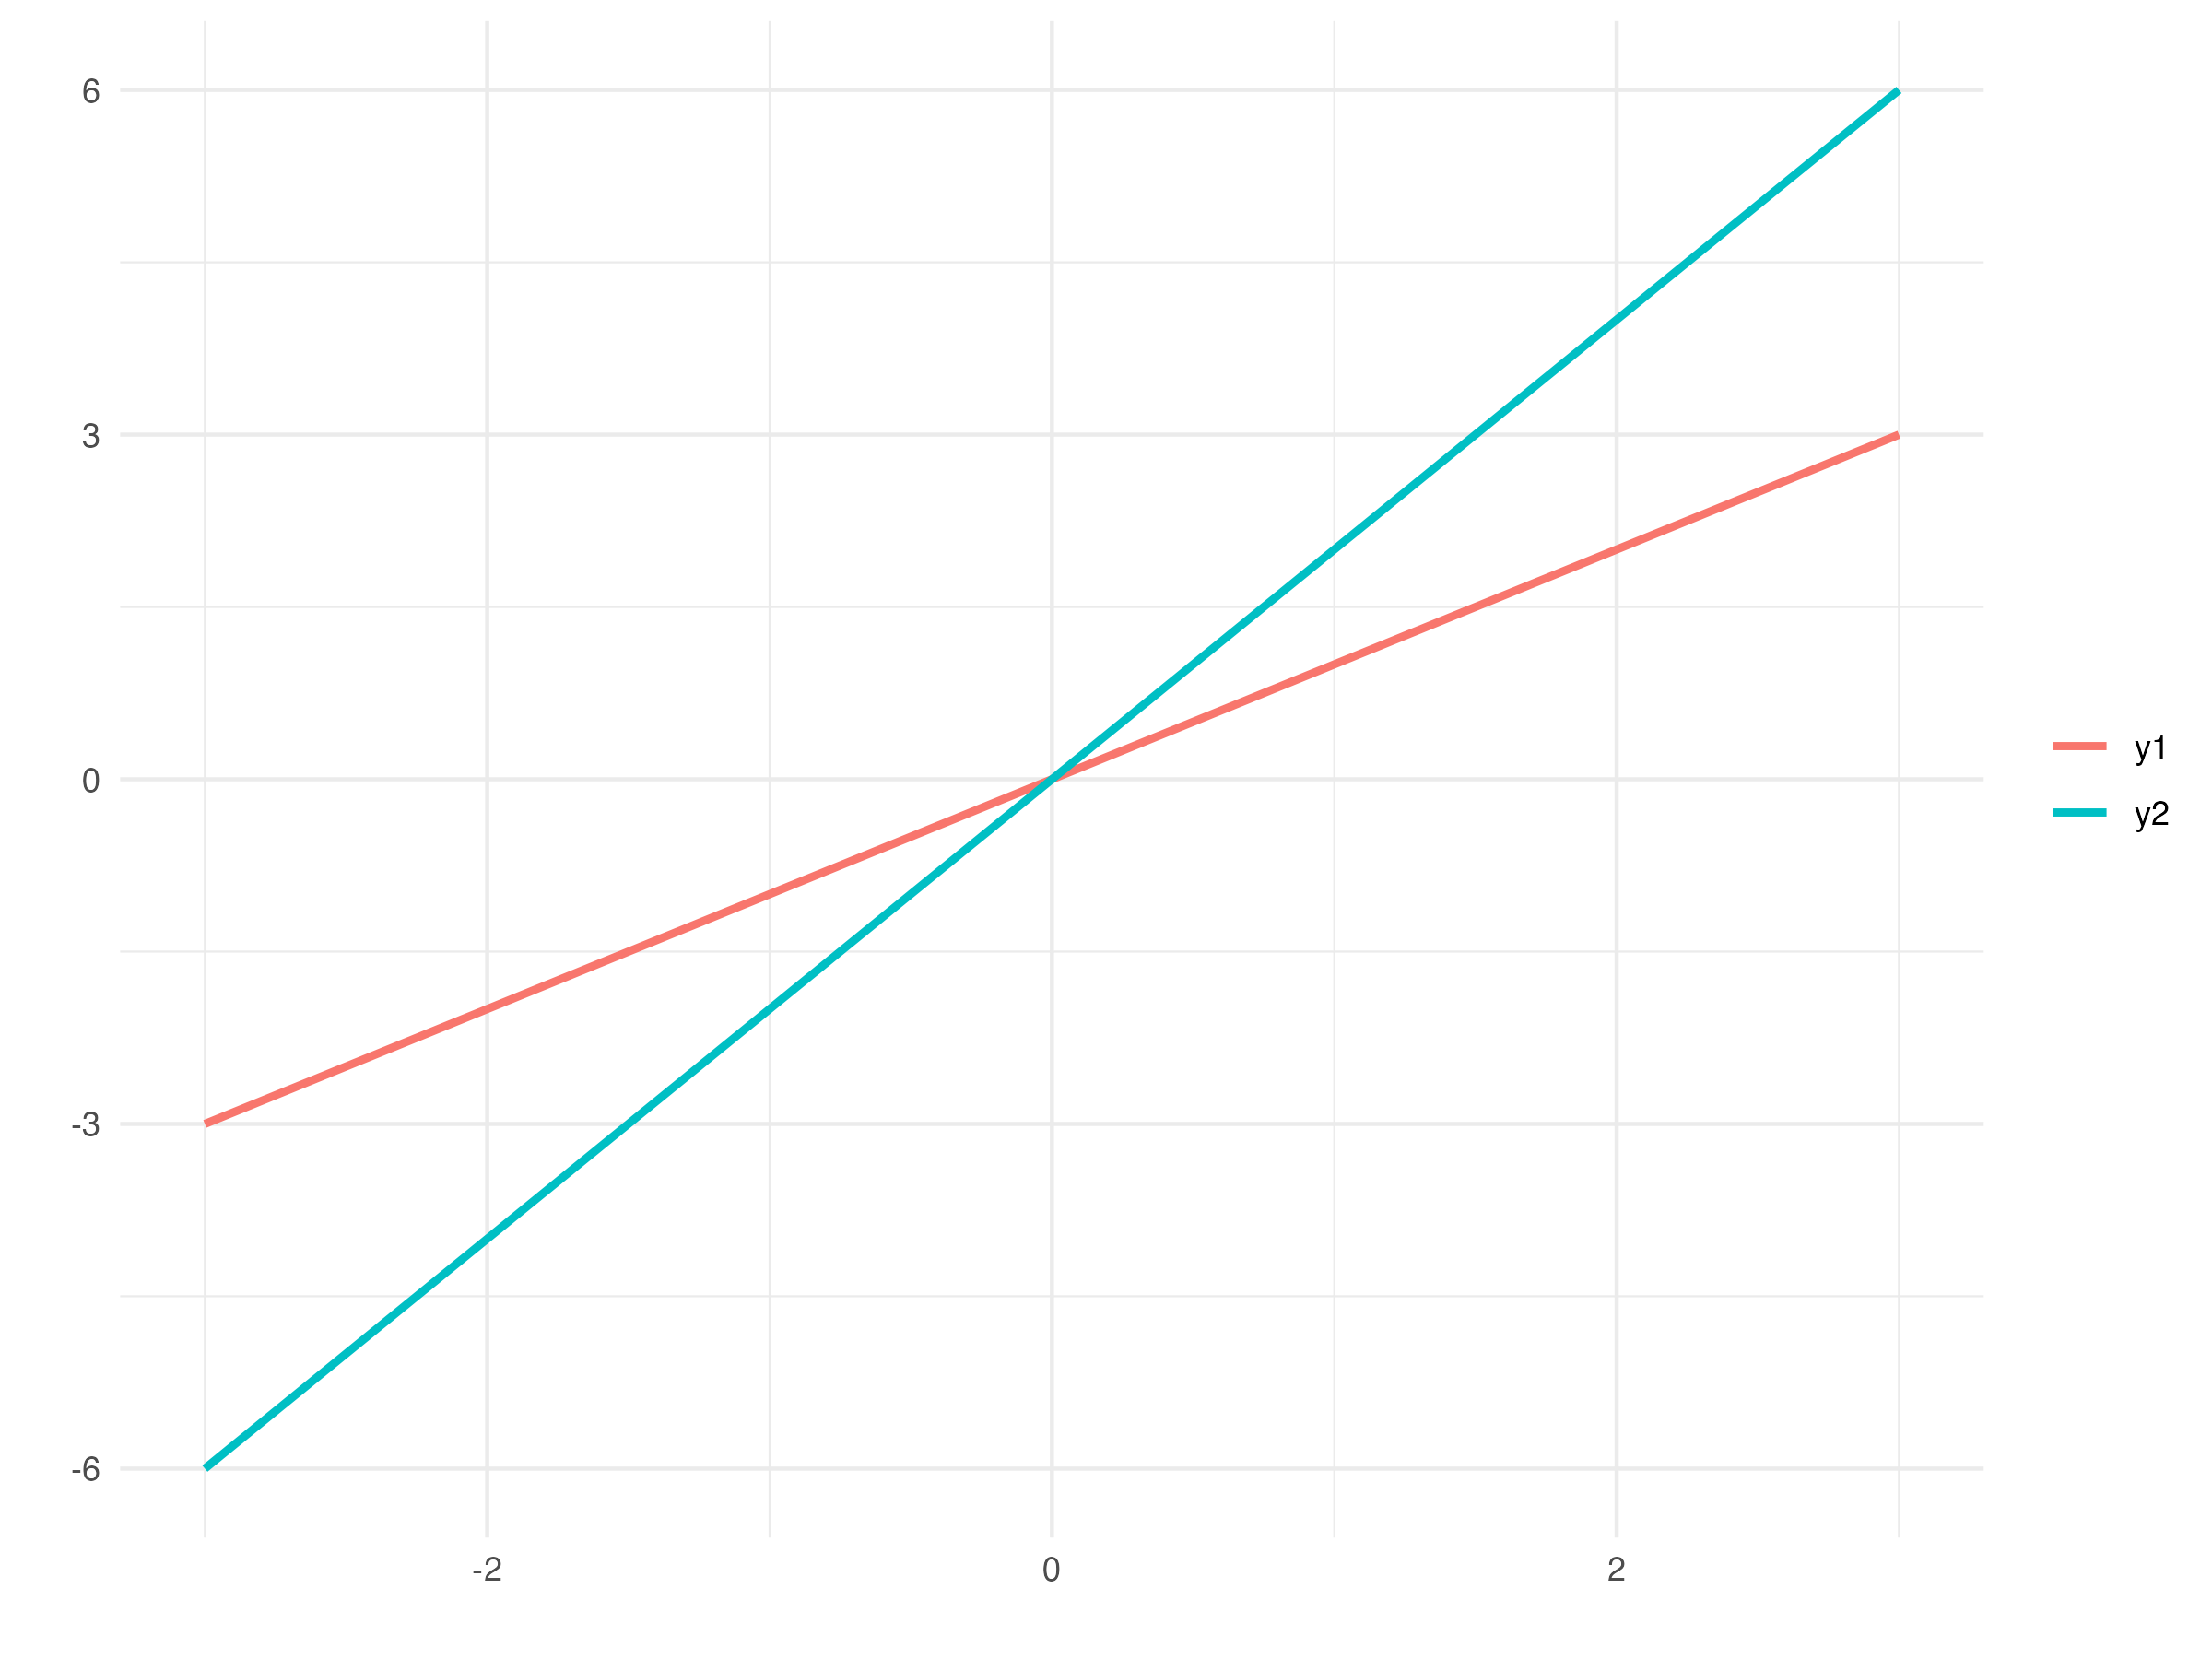
\includegraphics[width=\textwidth]{images/p_main_effect_ex1.png}
        \caption{Main terms as calculated via classical fANOVA for $g(x) = x_1 + 2 x_2 + x_1 x_2$.}
        \label{fig:main_effects_ex1}
    \end{minipage}%
    \hfill
    \begin{minipage}[t]{0.49\textwidth}
        \centering
        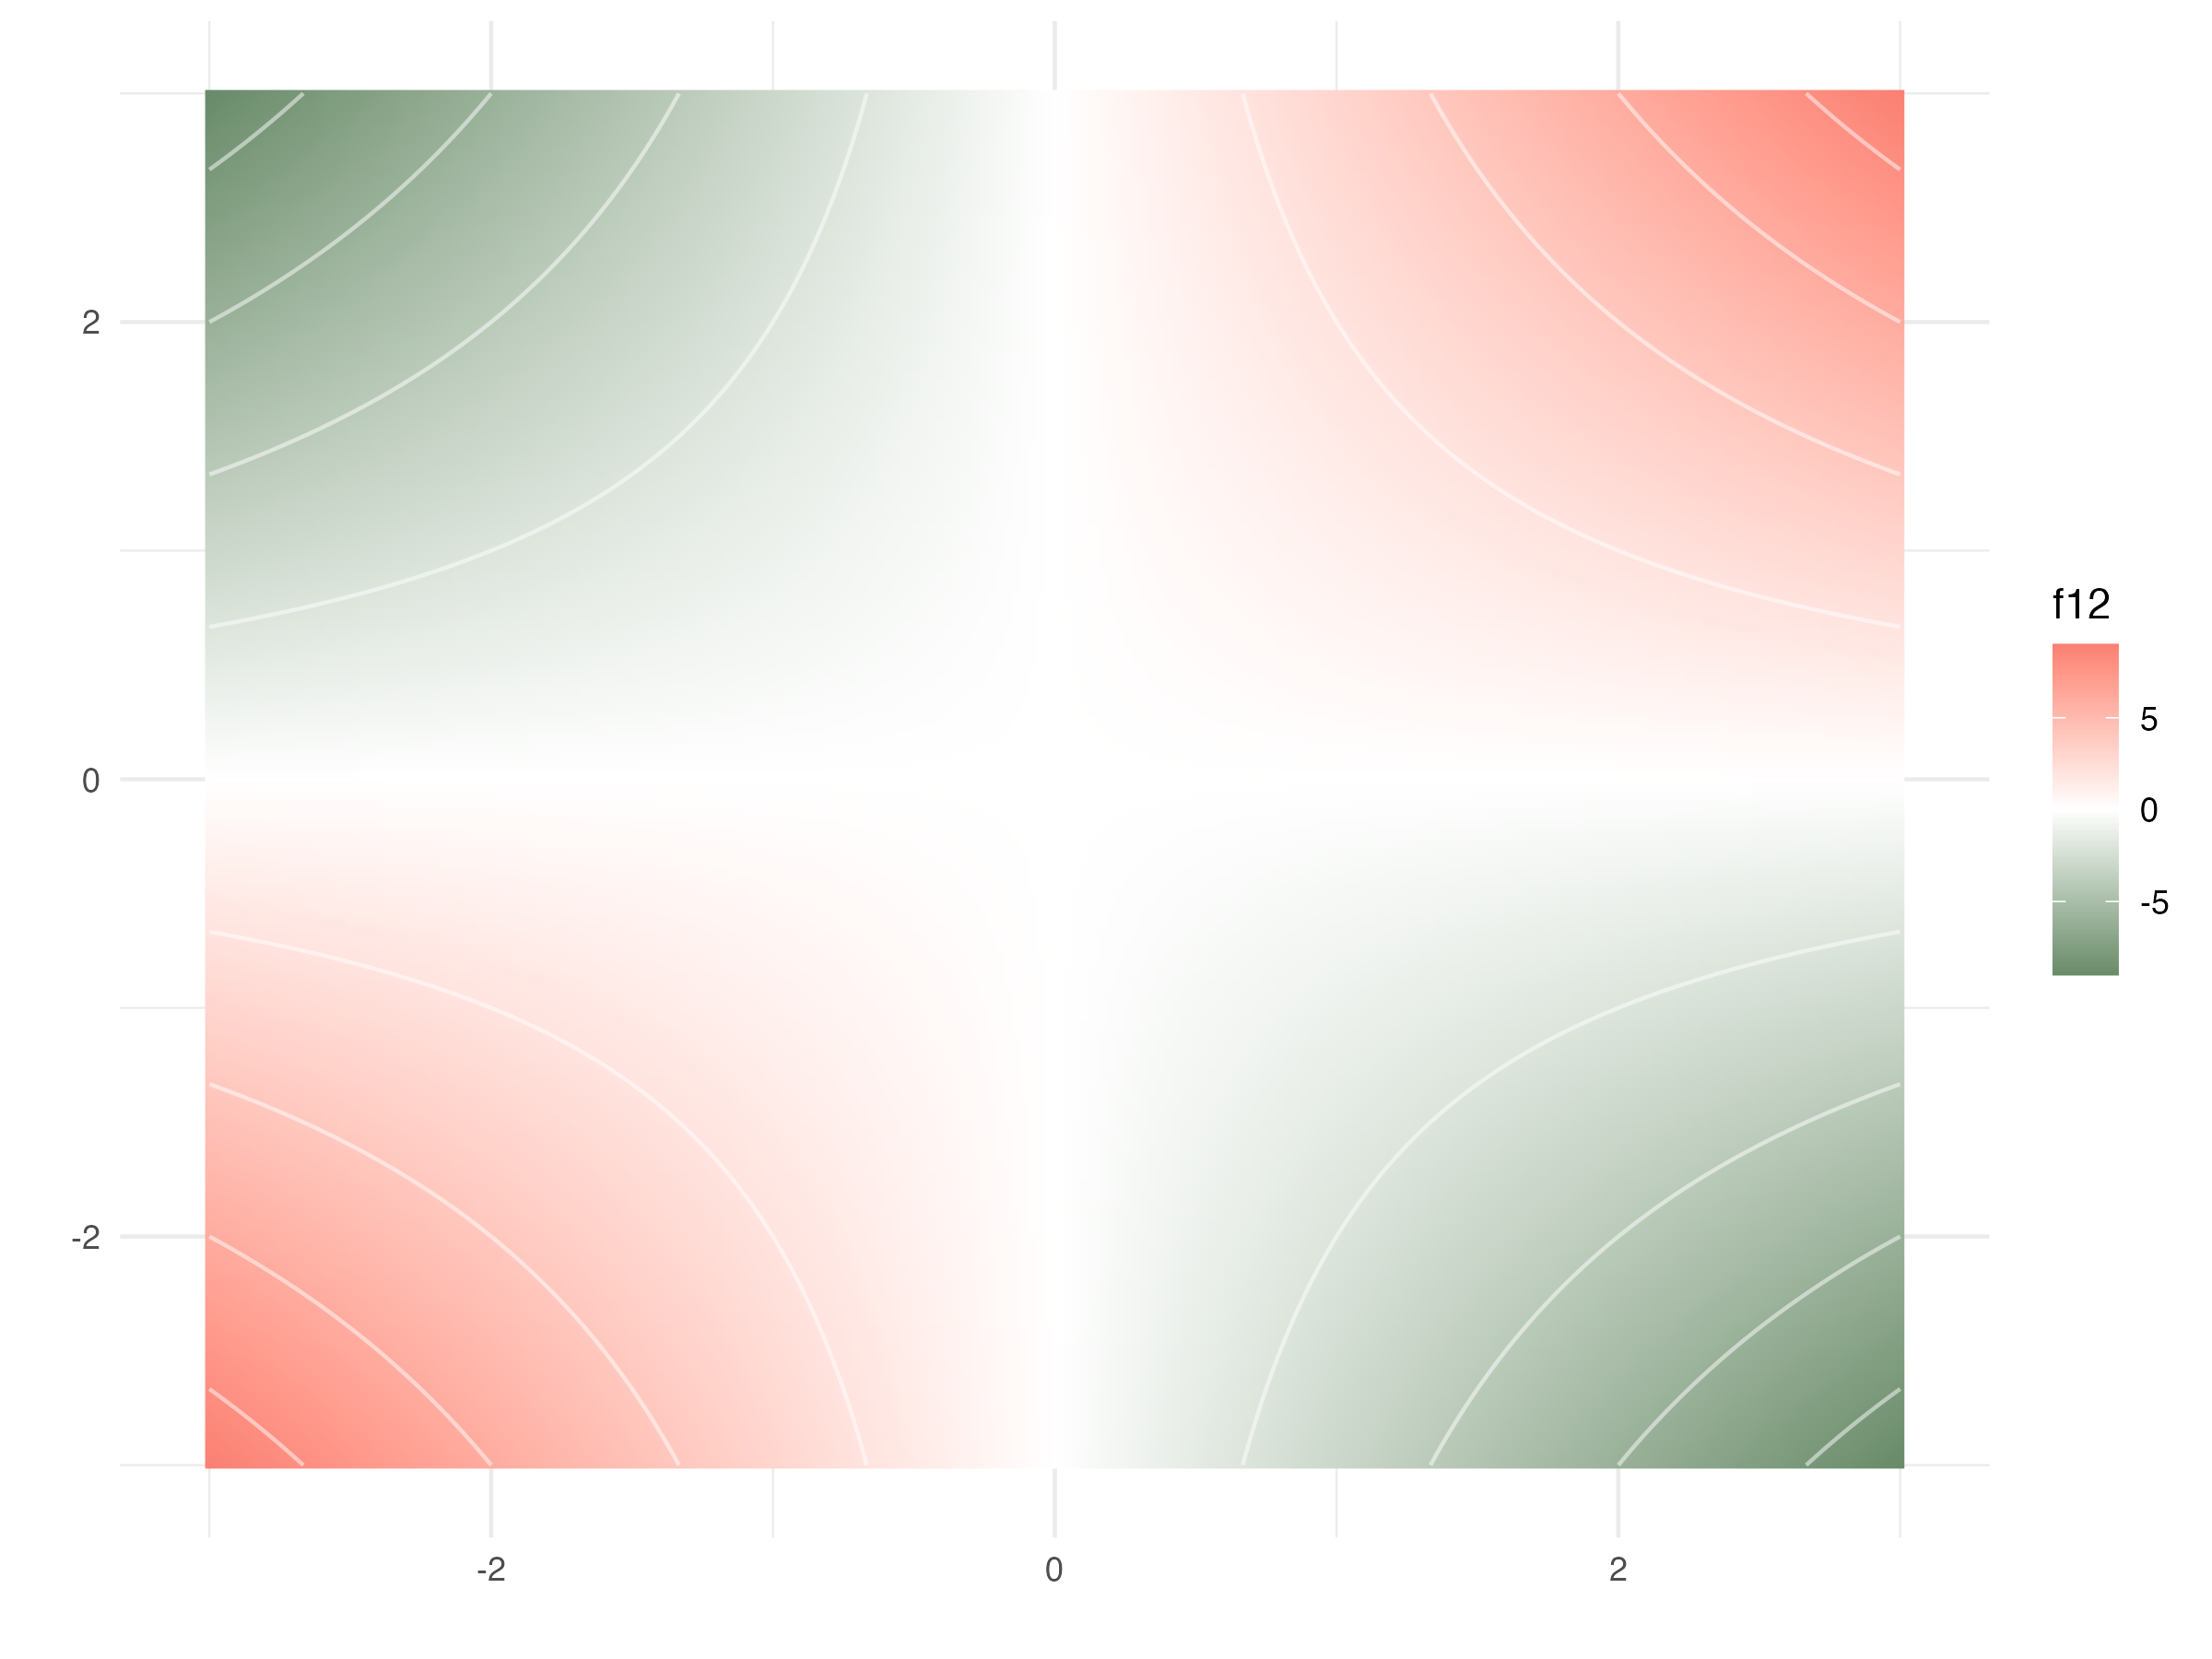
\includegraphics[width=\textwidth]{images/p_contour_ex1.png}
        \caption{Contour plot of $g(x) = x_1 + 2 x_2 + x_1 x_2$.}
        \label{fig:contour_ex1}
    \end{minipage}
\end{figure}

% Input: MVN, not centred, independent

% Input: Poisson/ Exponential/ Beta/ etc. not centred, independent


% Dependent inputs
We can compare them to the components we get under dependence from the ``naive'' approach.
% Zwei Plots für rho = 0.6 nebeneinander, jeweils halbe Breite
\begin{figure}[htpb]
    \centering
    \begin{minipage}[t]{0.49\textwidth}
        \centering
        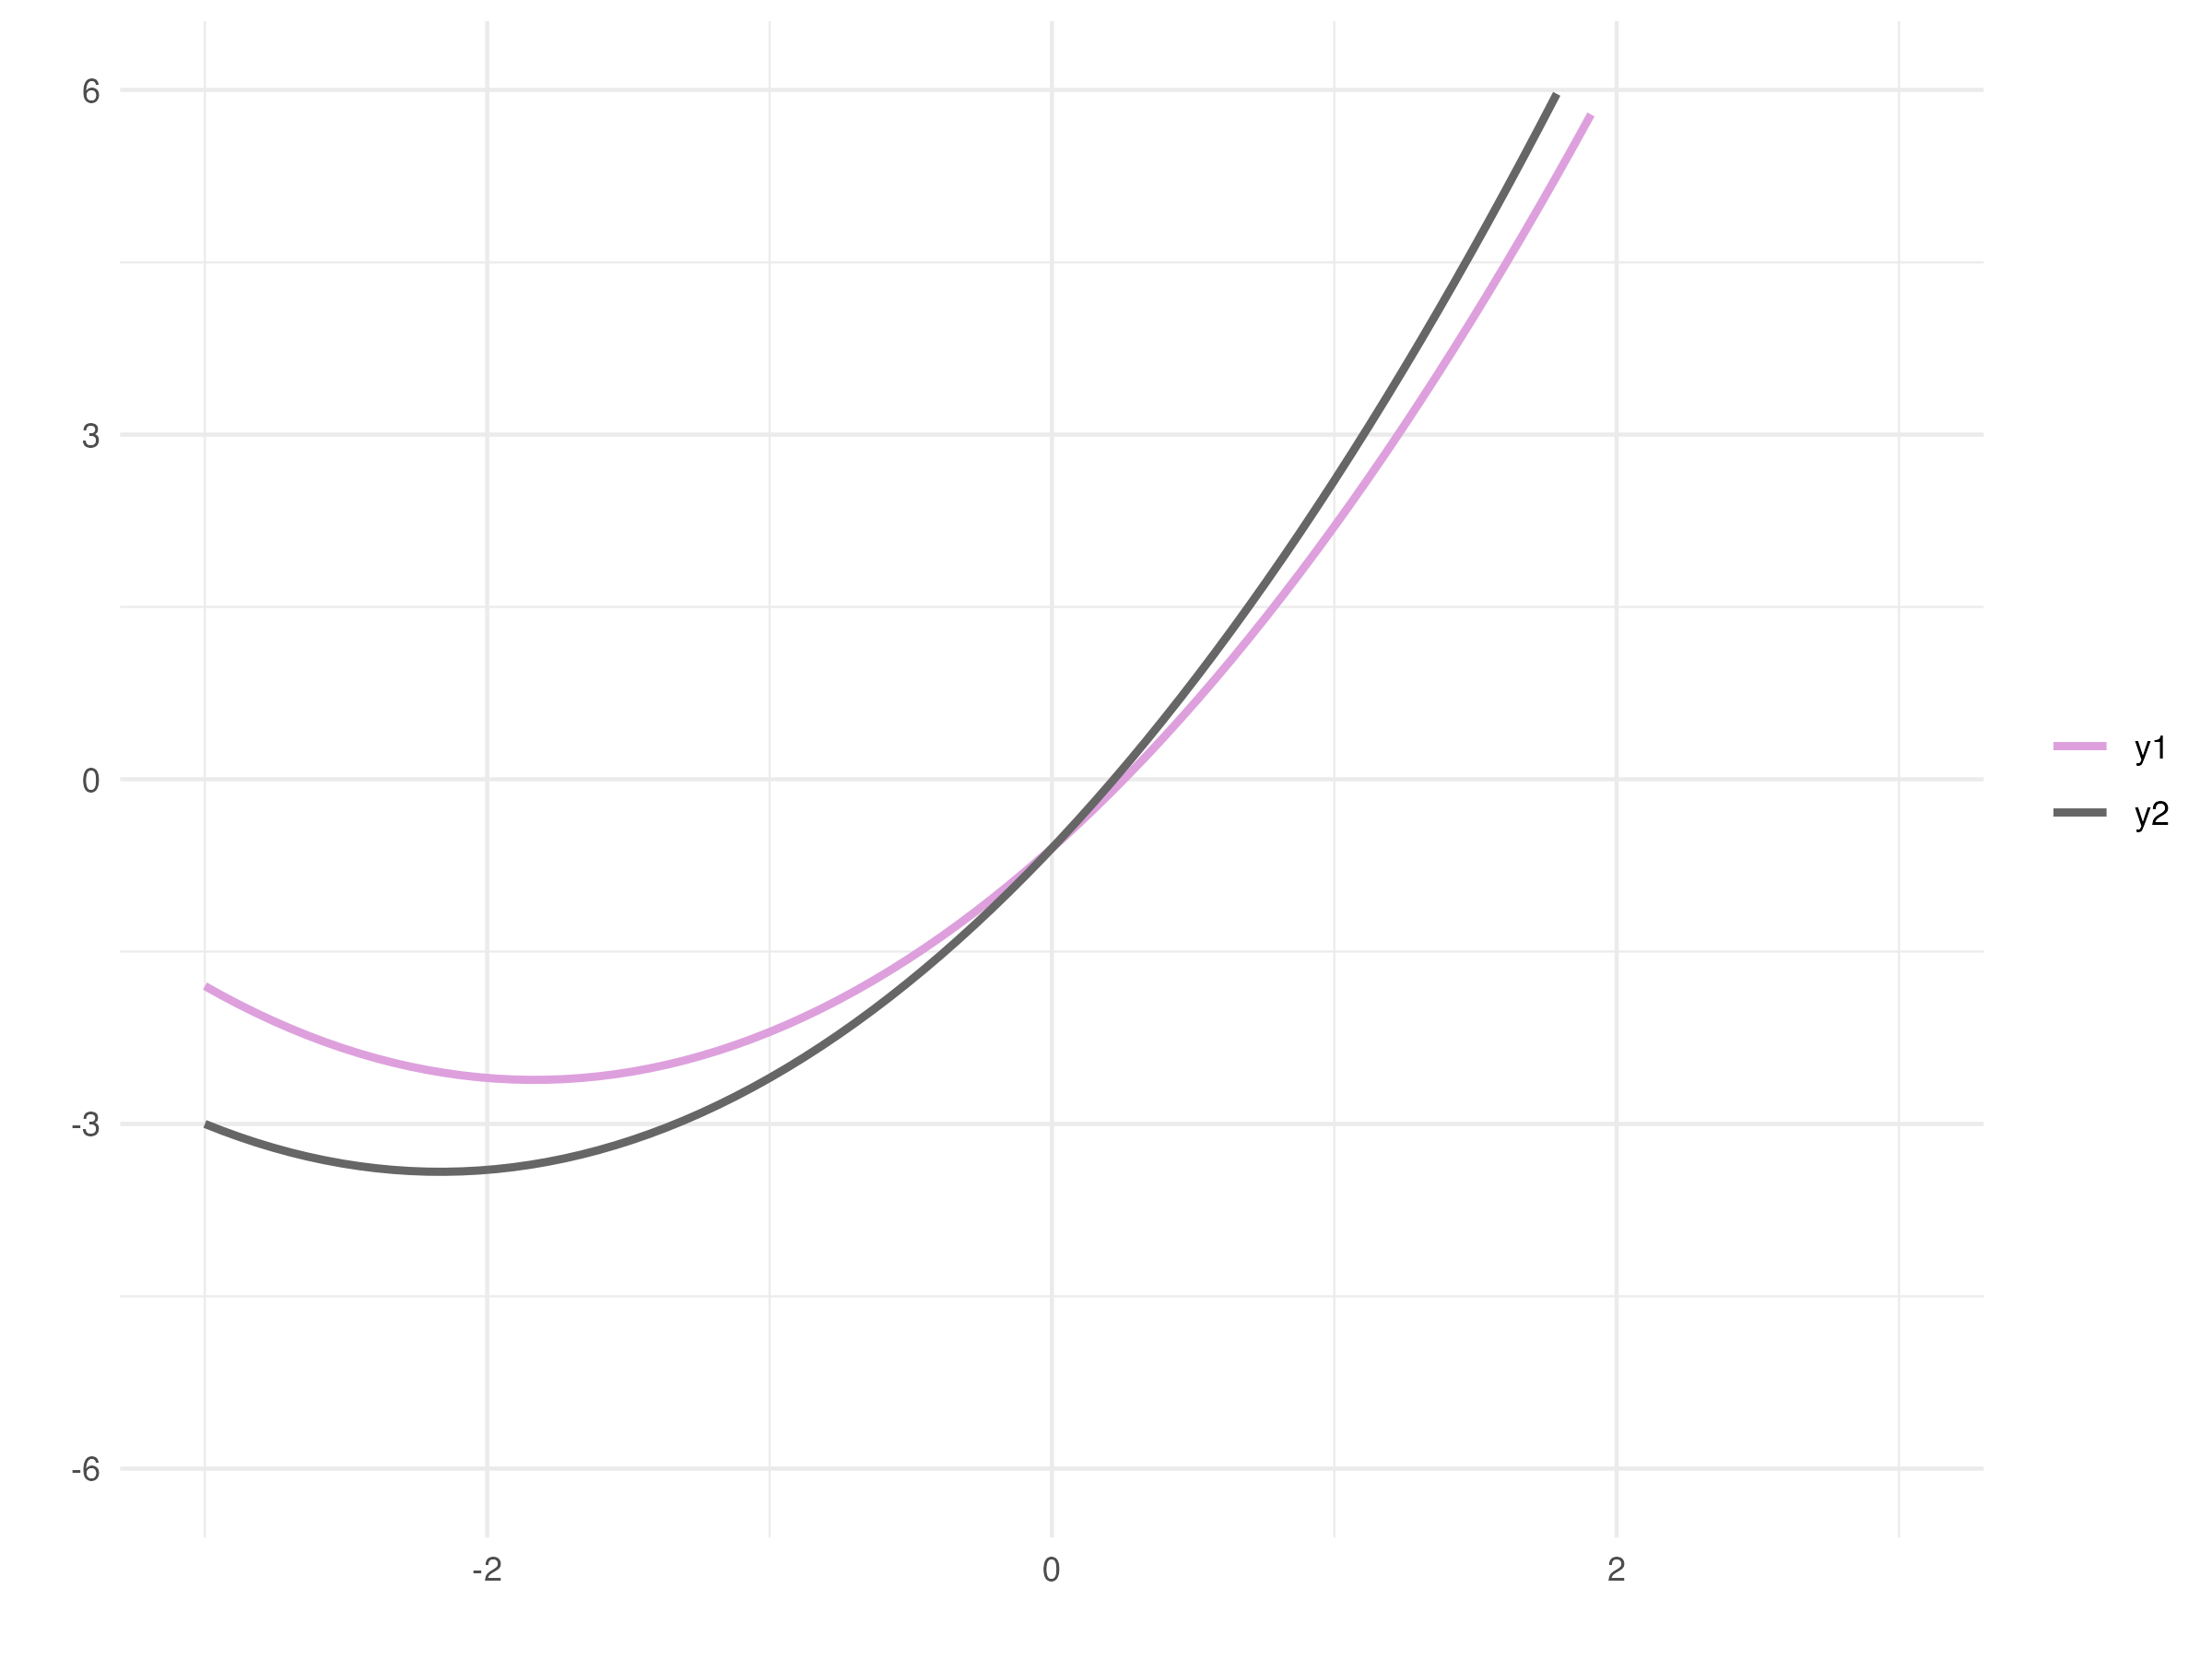
\includegraphics[width=\textwidth]{images/p_main_effect_ex1_rho06.png}
        \caption{Main terms as calculated via classical fANOVA for $g(x) = x_1 + 2 x_2 + x_1 x_2$ with $\rho = 0.6$.}
        \label{fig:main_effects_ex1_rho06}
    \end{minipage}%
    \hfill
    \begin{minipage}[t]{0.49\textwidth}
        \centering
        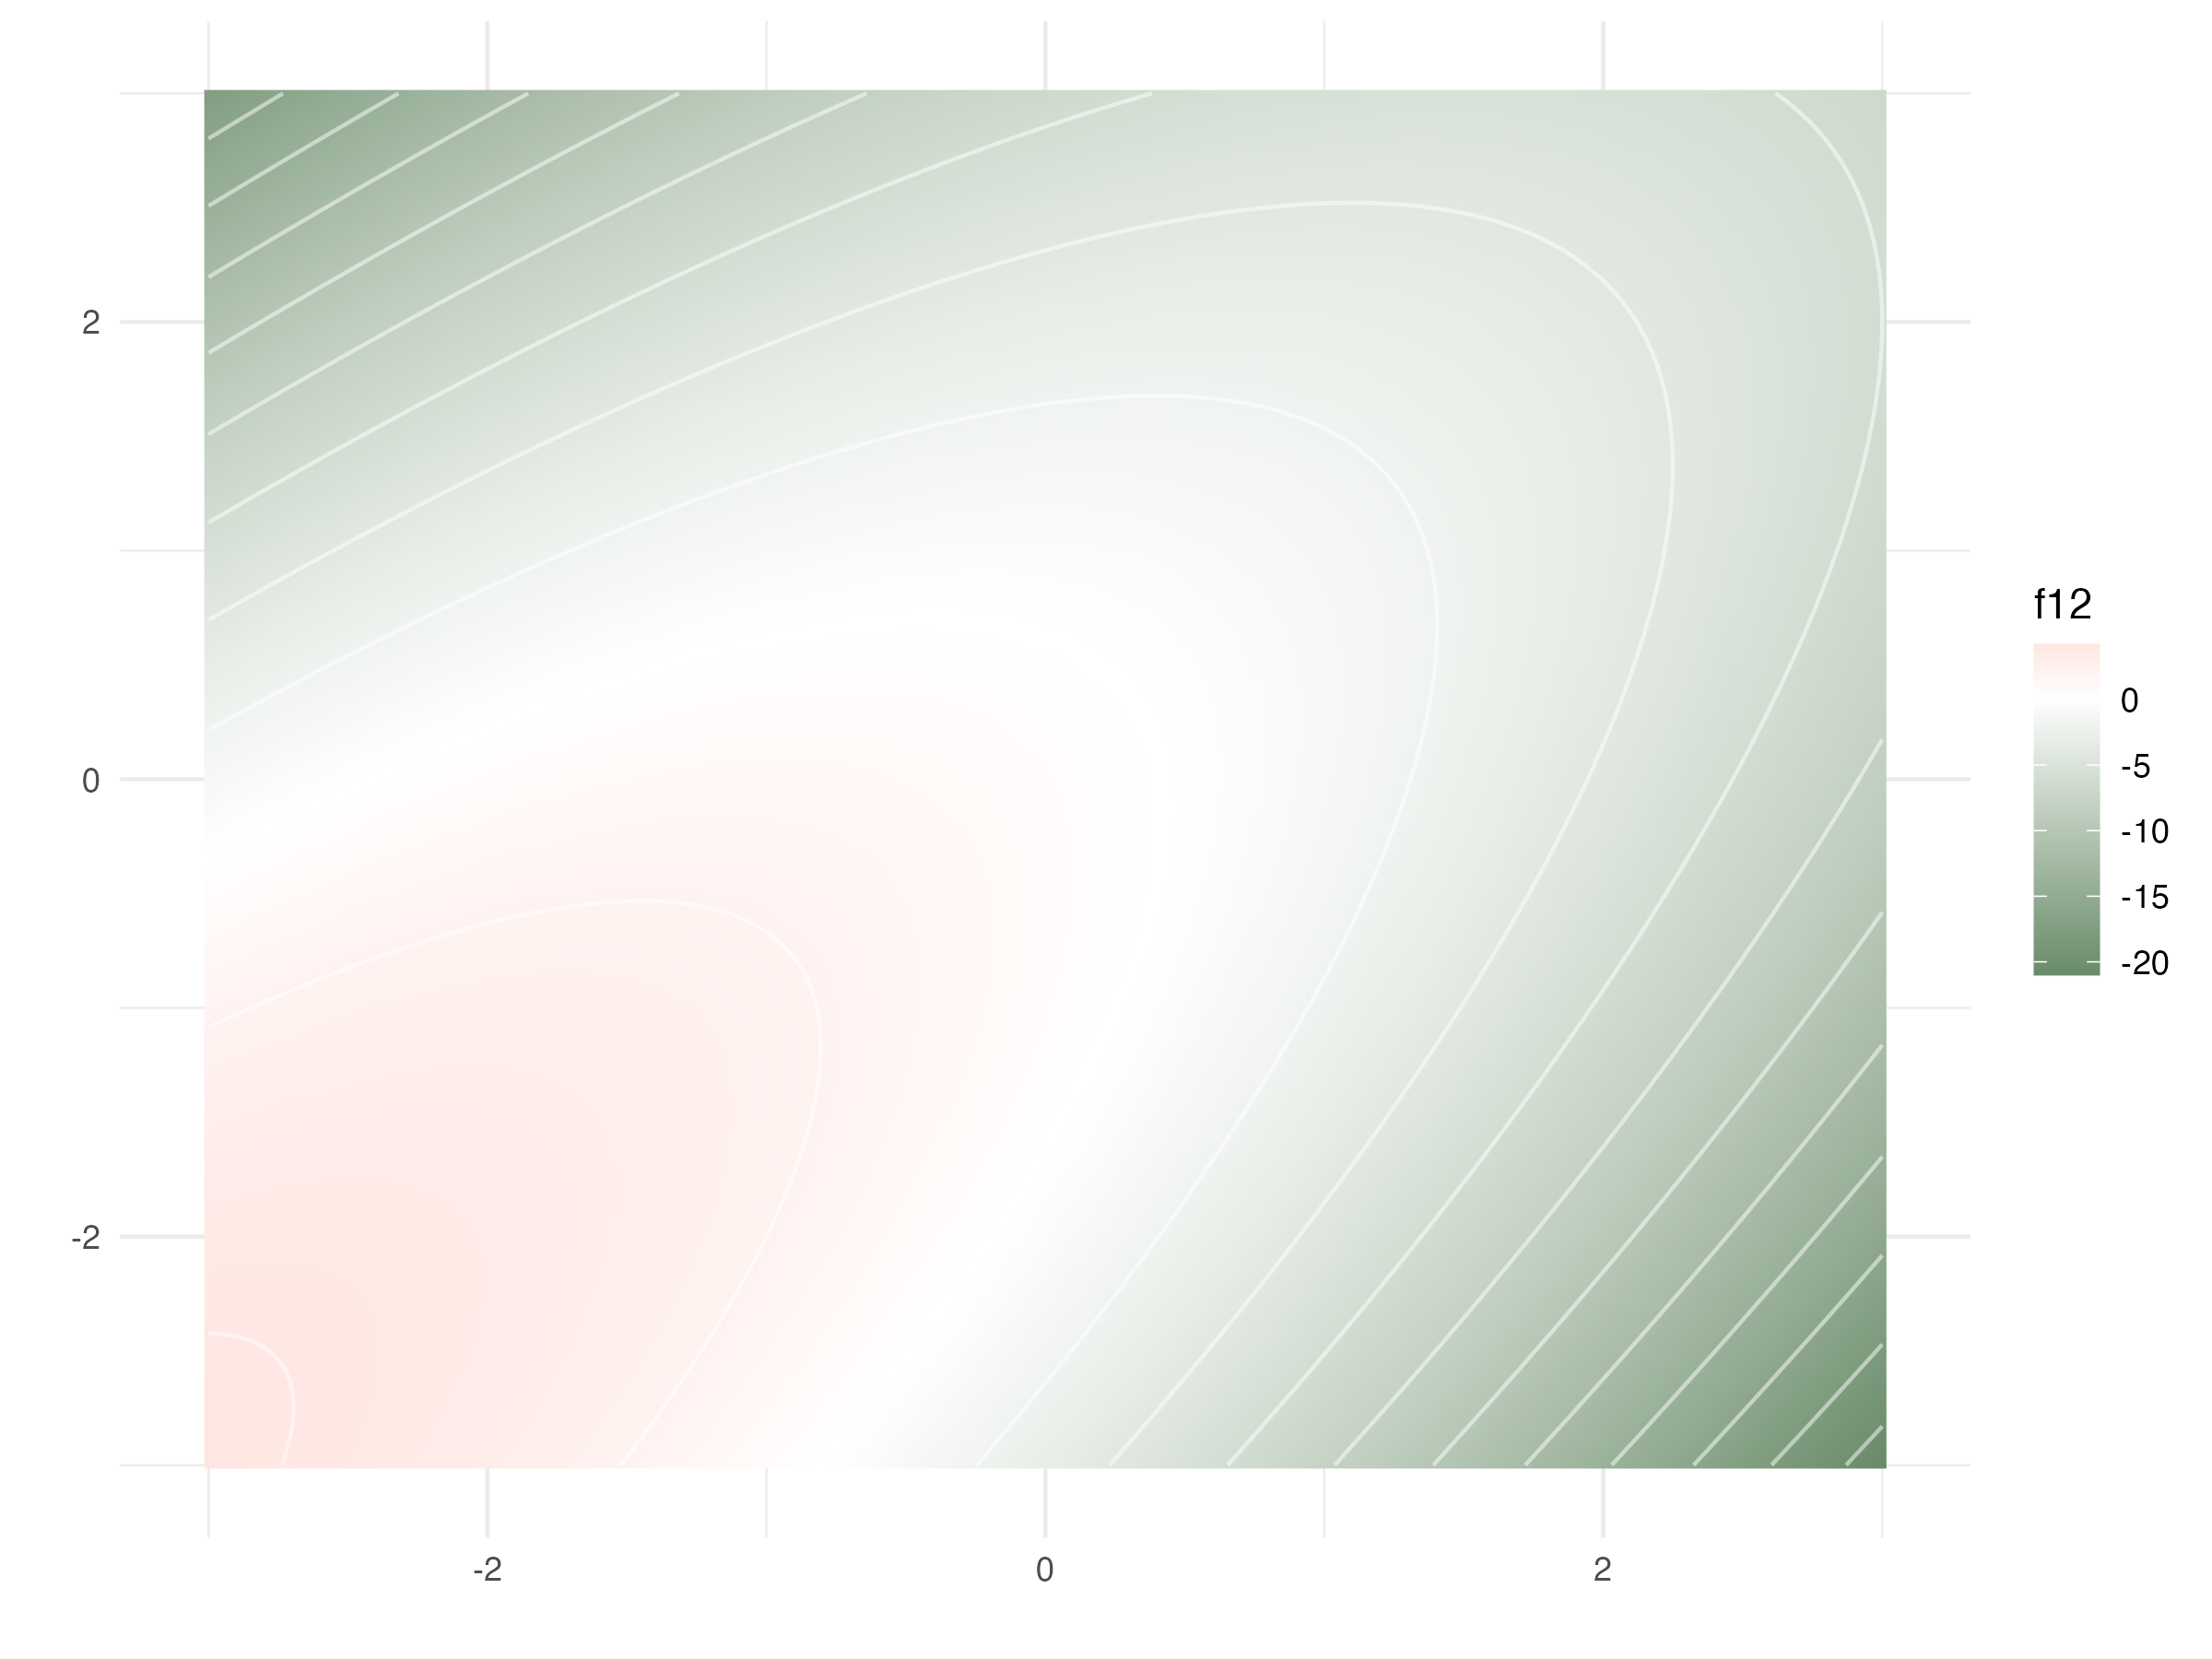
\includegraphics[width=\textwidth]{images/p_contour_ex1_rho06.png}
        \caption{Contour plot of $g(x) = x_1 + 2 x_2 + x_1 x_2$ with $\rho = 0.6$.}
        \label{fig:contour_ex1_rho06}
    \end{minipage}
\end{figure}

So \autoref{fig:main_effects_ex1_rho06} and \autoref{fig:contour_ex1_rho06} are not how we want the fANOVA components to look like under dependence - but how do we want them to look like?
Since we changed nothing about the structure of the function, should they generate identical plots as the classical components??

But on the other hand it cannot be that they give the same plots... I mean we wrote down the definition of the generalized components earlier, of course it is not the same as for the classical components. So as a function they literally look different. We couldn't compute them exactly but we could at least write out the system of equations we have to solve/ the probem that needs to be solved.
\section{Simulation Study}
% -----------------------------
% fANOVA Simulation Study Notes
% -----------------------------
% Baseline:
% Simple additive model with 1 interaction: f(x1, x2) = x1 + x2 + 0.5 * x1 * x2
% Inputs: x1, x2 ~ U(0,1), independent

% Simulation variants:
% 1. Input Distributions:
%    - Normal, exponential, log-normal, beta, Poisson, bimodal
% 2. Correlation:
%    - Use Gaussian copula to vary correlation (ρ ∈ [0, 0.9])
% 3. Functional Forms:
%    - Quadratic, exponential, sinusoidal, threshold (e.g. step/ReLU)
% 4. Noise:
%    - Add Gaussian noise ε ~ N(0, σ²), vary σ²
% 5. High-dimensional additive models:
%    - f(x) = x1 + x2² + log(x3+1) + sin(x4) with no interaction
% 6. Sparse interactions in many variables:
%    - Only a few interaction terms (e.g. x1*x2), rest irrelevant
% 7. Model misfit:
%    - Use approximate models (e.g., linear regressor on nonlinear function)
% 8. Compare with PDP and ALE:
%    - Use PDP/ALE for 1D/2D plots; explore where fANOVA gives better variance attribution

% Visualization:
% - Bar plots: variance shares per term
% - Line plots: interaction strength vs. correlation
% - Heatmaps: pairwise interaction strengths
% - Surface plots: function + components
% - Comparison: true vs estimated decomposition

% Design tips:
% - Use known ground truth
% - Fix seeds for repeatability
% - Use both analytic and model-based fANOVA
% -----------------------------

\subsection{Software implementations}
\begin{itemize}
    \item Suitable but currently problems installing locally: \href{https://github.com/frank-hutter/fanova?tab=readme-ov-file}{fanova}
    \item Context of kriging models; create own graphs (not super informative): \href{https://cran.r-project.org/web/packages/fanovaGraph/fanovaGraph.pdf?utm_source=chatgpt.com}{fanovaGraph}
    \item \href{https://rdrr.io/github/guillermozbta/mir/man/generateFunctionalANOVAData.html}{mlr3 function}
    \item \href{https://tntorch.readthedocs.io/en/latest/tutorials/anova.html}{tntorch}
    \item \href{https://pypi.org/project/shapiq/}{shapley values implementation python}
\end{itemize}

\label{simulation_study}
\newpage
% \section{Method Comparison}
% \label{iml_methods_comparison}
% This chapter will investigate the mathematical and conceptual parallels between fANOVA decomposition and other IML methods. Goal: get a better understanding for the role fANOVA plays in IML method landscape - When is it suitable? What are the advantages/ limitations compared to other methods?



\subsection{fANOVA and PD}
\cite{hooker2004} actually talks about parallels to PD in his first paper

\subsection{fANOVA and ALE}

\subsection{fANOVA and SHAP}
paper by \cite{andrewniianang2024}

\section{Conclusion}
\label{conclusion}

\section{Mathematical Statements}
\label{proofs}
\section*{Square Integrability of \( f_1(x_1) \)}

For now we want to show that the single fANOVA term \( f_1(x_1) \) is square integrable, given that the original function $f(x) \in \mathcal{L}^2$. We need to show that:
\[
\int |f_1(x_1)|^2 \, dx_1 < \infty
\]

The single fANOVA term is defined as:
\[
f_1(x_1) = \int f(x) \, dx_{-1} - f_0
\]

We take the squared norm, and integrate w.r.t. \( x_1 \) to use the Cauchy-Schwarz inequality:
\[
\int |f_1(x_1)|^2 \, dx_1 
= \int \left| \int f(x) \, dx_{-1} - f_0 \right|^2 dx_1
\]

\[
= \int | (\int f(x) \, dx_{-1})^2 
- 2 \int f(x) \, dx_{-1} f_0 
+ f_0^2 | dx_1
\]

Break this into three terms:
\begin{align*}
(1): &\quad \int \left| \int f(x) \, dx_{-1} \right|^2 dx_1 
\leq \int \left( \int 1^2 \, dx_{-1} \right) \left( \int |f(x)|^2 \, dx_{-1} \right) dx_1 
= \int |f(x)|^2 \, dx < \infty \\
\\
(2): &\quad 2 \int \left( \int f(x) \, dx_{-1} \right) f_0 \, dx_1 
= 2 f_0 \int \left( \int f(x) \, dx_{-1} \right) dx_1 
= 2 f_0^2 < \infty \\
\\
(3): &\quad \int f_0^2 \, dx_1 = f_0^2 < \infty
\end{align*}

Since each term (1)–(3) is finite, and \( \int |f_1(x_1)|^2 dx_1 \) is a linear combination of them: \(\int |f_1(x_1)|^2 dx_1 < \infty\)



% We want to show that the square integrability of the original function \( f \) implies the square integrability of the fANOVA terms \( f_0, f_1, \ldots, f_k \).
% For simplicity, we restrict ourselves to a fixed number of dimensions and therefore a fixed set of indices $i = 1, 2, 3, 4$.
% To start, we define the cumulative fANOVA decomposition as follows:
% \begin{align}
%     g_1(x) &= \int f(x) dx_{-1} = \int f(x) dx_2 dx_3 dx_4 \\
%     g_2(x) &= \int f(x) dx_{-2} = \int f(x) dx_1 dx_3 dx_4 \\
%     g_{1,2}(x) &= \int f(x) dx_{-1, -2} = \int f(x) dx_3 dx_4 \\
%     g_{1,2,3}(x) &= \int f(x) dx_{-1, -2, -3} = \int f(x) dx_4 \\
%     g_{1,2,3,4}(x) &= \int f(x) dx_{-1, -2, -3, -4} = \int f(x)
% \end{align}
% Further, recall that the Cauchy-Schwarz inequality for two function $f, g$ is given by:
% \begin{align}
%     \left( \int f(x) g(x) dx \right)^2 \leq \left( \int f(x)^2 dx \right) \left( \int g(x)^2 dx \right)
% \end{align}

% Let $f(x) \in L^2(\mathbb{R}^4)$ with $x = (x_1, x_2, x_3, x_4)$
% We want to show that the term $g_{1,2}$ is square integrable, i.e. $\int |g_{1,2}(x)|^2 dx < \infty$. The reasoning for other terms will follow the same principle.\par
% To be able to use Schwarz inequality, we square the norm of $g_{1,2}(x)$:
% \begin{align}
%     |g_{1,2}(x_1, x_2)|^2 
%     &= \left( \int f(x_1, x_2, x_3, x_4) \, dx_3 dx_4 \right)^2 \\
%     &\leq ( \int 1^2 \, dx_3 dx_4) (\int |f(x_1, x_2, x_3, x_4)|^2 \, dx_3 dx_4) \\
%     &= \int |f(x_1, x_2, x_3, x_4)|^2 \, dx_3 dx_4
% \end{align}
% The statement is true for fixed values of $x_1$ and $x_2$. To show that it holds for all $x_1, x_2$, we integrate over $x_1$ and $x_2$:
% \begin{align}
%     \int |g_{1,2}(x_1, x_2)|^2 \, dx_1 dx_2 
%     &\leq \int \left( \int |f(x_1, x_2, x_3, x_4)|^2 \, dx_3 dx_4 \right) \, dx_1 dx_2 \\
%     &= \int |f(x_1, x_2, x_3, x_4)|^2 \, dx \leq \infty
% \end{align}
% We used Fubini's theorem to write the sequential integration as a single integral over the whole space, which is valid under the assumption that $f$ is square integrable.
% As a last step, we use the square integrability of the cumulative fANOVA terms to show square integrability of the single fANOVA terms. We give an example for $f_{1,2}$:
% \begin{align}
%     f_{1,2}(x) &= g_{1,2}(x) - f_0 - f_1(x_1) - f_2(x_2) \\
%     &= g_{1,2}(x) - \int f(x) dx - \int f(x)\, dx_{-1} - \int f(x) dx_{-2} \\
%     &= g_{1,2}(x) - \int f(x) dx - g_1(x) - g_2(x) \leq \infty
% \end{align}
% Since all the terms in the last row are square integrable, we deal with a linear combination of square integrable functions, which is also square integrable.



\newpage

% ------------------------------------------------------------------------------
% APPENDIX ---------------------------------------------------------------------
% ------------------------------------------------------------------------------
    
\pagenumbering{Roman}

\setcounter{page}{5} % CHANGE

\appendix

\section{Appendix}
\label{app}
\section*{Square Integrability of \( f_1(x_1) \)}

For now we want to show that the single fANOVA term \( f_1(x_1) \) is square integrable, given that the original function $f(x) \in \mathcal{L}^2$. We need to show that:
\[
\int |f_1(x_1)|^2 \, dx_1 < \infty
\]

The single fANOVA term is defined as:
\[
f_1(x_1) = \int f(x) \, dx_{-1} - f_0
\]

We take the squared norm, and integrate w.r.t. \( x_1 \) to use the Cauchy-Schwarz inequality:
\[
\int |f_1(x_1)|^2 \, dx_1 
= \int \left| \int f(x) \, dx_{-1} - f_0 \right|^2 dx_1
\]

\[
= \int | (\int f(x) \, dx_{-1})^2 
- 2 \int f(x) \, dx_{-1} f_0 
+ f_0^2 | dx_1
\]

Break this into three terms:
\begin{align*}
(1): &\quad \int \left| \int f(x) \, dx_{-1} \right|^2 dx_1 
\leq \int \left( \int 1^2 \, dx_{-1} \right) \left( \int |f(x)|^2 \, dx_{-1} \right) dx_1 
= \int |f(x)|^2 \, dx < \infty \\
\\
(2): &\quad 2 \int \left( \int f(x) \, dx_{-1} \right) f_0 \, dx_1 
= 2 f_0 \int \left( \int f(x) \, dx_{-1} \right) dx_1 
= 2 f_0^2 < \infty \\
\\
(3): &\quad \int f_0^2 \, dx_1 = f_0^2 < \infty
\end{align*}

Since each term (1)–(3) is finite, and \( \int |f_1(x_1)|^2 dx_1 \) is a linear combination of them: \(\int |f_1(x_1)|^2 dx_1 < \infty\)



% We want to show that the square integrability of the original function \( f \) implies the square integrability of the fANOVA terms \( f_0, f_1, \ldots, f_k \).
% For simplicity, we restrict ourselves to a fixed number of dimensions and therefore a fixed set of indices $i = 1, 2, 3, 4$.
% To start, we define the cumulative fANOVA decomposition as follows:
% \begin{align}
%     g_1(x) &= \int f(x) dx_{-1} = \int f(x) dx_2 dx_3 dx_4 \\
%     g_2(x) &= \int f(x) dx_{-2} = \int f(x) dx_1 dx_3 dx_4 \\
%     g_{1,2}(x) &= \int f(x) dx_{-1, -2} = \int f(x) dx_3 dx_4 \\
%     g_{1,2,3}(x) &= \int f(x) dx_{-1, -2, -3} = \int f(x) dx_4 \\
%     g_{1,2,3,4}(x) &= \int f(x) dx_{-1, -2, -3, -4} = \int f(x)
% \end{align}
% Further, recall that the Cauchy-Schwarz inequality for two function $f, g$ is given by:
% \begin{align}
%     \left( \int f(x) g(x) dx \right)^2 \leq \left( \int f(x)^2 dx \right) \left( \int g(x)^2 dx \right)
% \end{align}

% Let $f(x) \in L^2(\mathbb{R}^4)$ with $x = (x_1, x_2, x_3, x_4)$
% We want to show that the term $g_{1,2}$ is square integrable, i.e. $\int |g_{1,2}(x)|^2 dx < \infty$. The reasoning for other terms will follow the same principle.\par
% To be able to use Schwarz inequality, we square the norm of $g_{1,2}(x)$:
% \begin{align}
%     |g_{1,2}(x_1, x_2)|^2 
%     &= \left( \int f(x_1, x_2, x_3, x_4) \, dx_3 dx_4 \right)^2 \\
%     &\leq ( \int 1^2 \, dx_3 dx_4) (\int |f(x_1, x_2, x_3, x_4)|^2 \, dx_3 dx_4) \\
%     &= \int |f(x_1, x_2, x_3, x_4)|^2 \, dx_3 dx_4
% \end{align}
% The statement is true for fixed values of $x_1$ and $x_2$. To show that it holds for all $x_1, x_2$, we integrate over $x_1$ and $x_2$:
% \begin{align}
%     \int |g_{1,2}(x_1, x_2)|^2 \, dx_1 dx_2 
%     &\leq \int \left( \int |f(x_1, x_2, x_3, x_4)|^2 \, dx_3 dx_4 \right) \, dx_1 dx_2 \\
%     &= \int |f(x_1, x_2, x_3, x_4)|^2 \, dx \leq \infty
% \end{align}
% We used Fubini's theorem to write the sequential integration as a single integral over the whole space, which is valid under the assumption that $f$ is square integrable.
% As a last step, we use the square integrability of the cumulative fANOVA terms to show square integrability of the single fANOVA terms. We give an example for $f_{1,2}$:
% \begin{align}
%     f_{1,2}(x) &= g_{1,2}(x) - f_0 - f_1(x_1) - f_2(x_2) \\
%     &= g_{1,2}(x) - \int f(x) dx - \int f(x)\, dx_{-1} - \int f(x) dx_{-2} \\
%     &= g_{1,2}(x) - \int f(x) dx - g_1(x) - g_2(x) \leq \infty
% \end{align}
% Since all the terms in the last row are square integrable, we deal with a linear combination of square integrable functions, which is also square integrable.

\newpage

\section{Electronic appendix}
\label{el_app}

Data, code and figures are provided in electronic form.

\newpage
    
% ------------------------------------------------------------------------------
% BIBLIOGRAPHY -----------------------------------------------------------------
% ------------------------------------------------------------------------------

\RaggedRight
\bibliography{bibliography_2, bibliography_manual}
\bibliographystyle{dcu}
\newpage

% ------------------------------------------------------------------------------
% DECLARATION OF AUTHORSHIP-----------------------------------------------------
% ------------------------------------------------------------------------------

\Large
\noindent
\textbf{Declaration of authorship} 
\vspace{0.5cm}
\noindent
\normalsize

I hereby declare that the report submitted is my own unaided work. All direct 
or indirect sources used are acknowledged as references. I am aware that the 
Thesis in digital form can be examined for the use of unauthorized aid and in 
order to determine whether the report as a whole or parts incorporated in it may 
be deemed as plagiarism. For the comparison of my work with existing sources I 
agree that it shall be entered in a database where it shall also remain after 
examination, to enable comparison with future Theses submitted. Further rights 
of reproduction and usage, however, are not granted here. This paper was not 
previously presented to another examination board and has not been published.
\\

\vspace{1cm}
\textcolor{orange}{Location, date} \\

\vspace{3cm}

\noindent\rule{0.5\textwidth}{0.4pt} \\

\textcolor{orange}{Name}

% ------------------------------------------------------------------------------

\end{document}
